%==============================================================================
% Importando a classe
%==============================================================================
\documentclass{templufla}          

%==============================================================================
% Pacote hyperref para referências cruzadas dentro do documento \ref e \autoref
% O pacote hyperref precisa ser importado o mais cedo possível.

% Setspace precisa estar antes do hyperref para usar a versão atual do abntex.
\usepackage{setspace}

% Definindo cores para os links cruzados
\usepackage{xcolor}              % para mais cores
\definecolor{rltred}{rgb}{0.2,0,0}
\definecolor{rltgreen}{rgb}{0,0.2,0}
\definecolor{rltblue}{rgb}{0,0,0.2}


% Importa hyperref
\usepackage[%
hidelinks, % colorlinks=true, | Troque se quiser link com cor
urlcolor=rltblue,       % \href{...}{...} external (URL)
filecolor=rltgreen,     % \href{...} local file
linkcolor=rltred,       % \ref{...} and \pageref{...}
citecolor=rltgreen,%
]{hyperref} % 


%==============================================================================
% Configurando a linguagem do template

% Português
\usepackage[brazilian]{babel}
% Adaptando os nomes das seções
\addto\captionsbrazil{
	\renewcommand{\chaptername}{Seção}
	\renewcommand{\subsectionname}{Seção}
	\renewcommand{\subsubsectionname}{Seção}
}
\addto\extrasbrazil{
	\renewcommand{\chapterautorefname}{Seção}
	\renewcommand{\subsectionautorefname}{Seção}
	\renewcommand{\subsubsectionautorefname}{Seção}
}

% Inglês
%\usepackage[english]{babel}
%% Adapta nomes de seção
\addto\captionsenglish{
	\renewcommand{\chaptername}{Section}
	\renewcommand{\subsectionname}{Section}
	\renewcommand{\subsubsectionname}{Section}
}
\addto\extrasenglish{
	\renewcommand{\chapterautorefname}{Section}
	\renewcommand{\subsectionautorefname}{Section}
	\renewcommand{\subsubsectionautorefname}{Section}
}

% Adaptar nomes fixos

% títulos de pessoa
\renewcommand{\orientadorname}{Advisor}
\renewcommand{\orientadoraname}{Advisor}
\renewcommand{\coorientadorname}{Co-advisor}
\renewcommand{\coorientadoraname}{Co-advisor}

% títulos
\renewcommand{\agradecimentosname}{Acknowledgments}
\renewcommand{\listadefigurasname}{List of Figures}
\renewcommand{\listadeilustracoesname}{List of Illustrations}
\renewcommand{\listadegraficosname}{List of Plots}
\renewcommand{\listadetabelasname}{List of Tables}
\renewcommand{\listadequadrosname}{List of Frames}
\renewcommand{\listadeexemplosname}{List of Examples}
\renewcommand{\listadeteoremasname}{List of Theorems}
\renewcommand{\listadeabreviaturasname}{List of Abbreviations}
\renewcommand{\listadesiglasname}{List of Acronyms}
\renewcommand{\listadesimbolosname}{List of Symbols}
\renewcommand{\referenciasname}{References}
\renewcommand{\glossarioname}{Glossary}
\renewcommand{\anexosname}{Annexes}
\renewcommand{\apendicesname}{Appendixes}
\renewcommand{\indicename}{Index}


% elementos
\renewcommand{\ilustracaoname}{Illustration}
\renewcommand{\graficoname}{Plot}
\renewcommand{\quadroname}{Frame}
\renewcommand{\exemploname}{Example}
\renewcommand{\teoremaname}{Theorem}
\renewcommand{\anexoname}{Annex}
\renewcommand{\apendicename}{Appendix}

% geral
\renewcommand{\fontename}{Source}
\renewcommand{\aprovadaemname}{ACCEPTED on }

%==============================================================================
% Configuração dos pacotes necessários
% Primeiros pacotes (alguns precisam ser importados depois)

% TEXTOS
\usepackage[T1]{fontenc}         % usa fontes postscript com acentos
\usepackage[utf8]{inputenc}      % permite edição direta com acentos
\usepackage{listings}            % para inserção de código
\usepackage{fancyvrb}            % para inserção de saídas de comandos

% MATEMÁTICA
\usepackage{amsmath}             % pacote da AMS para Matemática Avançada
\usepackage{amssymb}             % símbolos extras da AMS
\usepackage{mathtools}			 % para mais comandos de matemática
\usepackage{latexsym}            % símbolos extras do LaTeX

% TABELAS
\usepackage{longtable}           % para tabelas muito grandes
\usepackage{array}               % para mais opções em tabelas
%\usepackage{colortbl} % removido: incompativel com array 2.5g no MiKTeX 24.1
\usepackage{multirow}            % para células com várias linhas
\usepackage{multicol}            % para células com várias colunas

% FIGUAS E GRÁFICOS
\usepackage{subfigure}           % para figuras dentro de figuras
\usepackage{caption}             % para remodelar o formato dos títulos


%==============================================================================
% Citações/referências no formato ABNT, utilizando o pacote abntex2.
% O pacote já vem na maioria das distribuições (texLive, MikTeX, Overleaf e etc...)
% mas, caso você seja super roots e não use os listados, precisa instalar o abntex2:
% http://abntex.codigolivre.org.br/

% A versão disponível com esse template sofreu algumas alterações para se adaptar ao
% padrão atual, já que a original está desatualizada.
% Para mais informações, vizite o repositório oficial do template.


% abnt-emphasize=bf coloca o título das bibliografias em negrito
% abnt-etal-list=3 limita o número de autores antes de et al. para 3
% abnt-url-package=xurl diz para usar o pacote url
\usepackage[alf, abnt-etal-list=3, abnt-emphasize=bf]{abntex2cite}

%==============================================================================
% Ajustando os pacotes importados

% Definindo cores para elementos tabulares
%\newcolumntype{Z}{|>{\columncolor[gray]{0.9}}l|} %cor cinza em células
% Definicoes do template substituidas: a versao original (m{} com let-newline)
% falha com o pacote array atual (MiKTeX 24.1). Versao com p{}.
\newcolumntype{L}[1]{>{\raggedright\arraybackslash}p{#1}}
\newcolumntype{C}[1]{>{\centering\arraybackslash}p{#1}}
\newcolumntype{R}[1]{>{\raggedleft\arraybackslash}p{#1}}

% Definindo espaçamento vertical de elementos tabulares
\renewcommand{\arraystretch}{1.5}

% Configuração padrão do listings (ambiente de código)
\lstset{
	extendedchars=true,
	breaklines=true,
	tabsize=3,
	basicstyle=\linespread{1}\ttfamily\normalsize,
	stringstyle=\em,
	showstringspaces=true,
	inputencoding=utf8,
	captionpos=t,
	backgroundcolor=\color{black!5},
	literate={{á}{{\'a}}1 {é}{{\'e}}1 {í}{{\'i}}1 {ó}{{\'o}}1 {ú}{{\'u}}1
	{Á}{{\'A}}1 {É}{{\'E}}1 {Í}{{\'I}}1 {Ó}{{\'O}}1 {Ú}{{\'U}}1
	{â}{{\^a}}1 {ê}{{\^e}}1 {ô}{{\^o}}1
	{Â}{{\^A}}1 {Ê}{{\^E}}1 {Ô}{{\^O}}1
	{ã}{{\~a}}1 {õ}{{\~o}}1 {ẽ}{{\~e}}1 
	{ç}{{\c{c}}}1
	{à}{{\`{a}}}1{À}{{\`{A}}}1}
}

% Carregamento do glossário, listas de siglas, símbolos e etc
\loadglsentries{glossarios/abreviaturas}
\loadglsentries{glossarios/glossario}
\loadglsentries{glossarios/siglas}
\loadglsentries{glossarios/simbolos}

% Especificando hifenizações que por ventura LaTeX não saiba fazer
% Por padrão 99,9% dos termos em português devem ser hifenizados corretamente.
% Adicione aqui palavras precise especificar como hifenizar (ou não hifenizar)
\hyphenation{software am-bien-te coor-de-na-ção FAE-PE TelEduc Williams UFLA Murray Bookchin}

%==============================================================================
% Dados da monografia, capa: autor, titulo, banca, etc... - SUBSTITUA DE ACORDO
%==============================================================================
% Dados para o arquivo PDF (metadados)

\hypersetup{%
% Titulo
pdftitle={AgroVisible: Ferramenta de Apoio Prescritivo à Decisão Baseada em Aprendizado Profundo e Programação Dinâmica para Maximização do Lucro do Cafeicultor},
% Autor
pdfauthor={Alexandre Marques Spinola Cardoso},
% Descrição
pdfsubject={Trabalho de Conclusão de Curso},
% Palavras-Chave
pdfkeywords={café arábica; LSTM; programação dinâmica; sistema de apoio à decisão; comercialização agrícola.}
}
	
%==============================================================================
% Informações básicas

% Nome da(s)/do(s) autora(s)/autor(es)
\author{Alexandre Marques Spinola Cardoso}

% Título do trabalho, em lígua vernácula
\title{AgroVisible: Ferramenta de Apoio Prescritivo à Decisão Baseada em Aprendizado Profundo e Programação Dinâmica para Maximização do Lucro do Cafeicultor}

% Subítulo do trabalho, em lígua vernácula
%\subtitle{}

% Título do trabalho, em inglês
\engtitle{AgroVisible: A Prescriptive Decision Support Tool Based on Deep Learning and Dynamic Programming for Maximizing Coffee Grower Profit}

% Subítulo do trabalho, em inglês
%\engsubtitle{}

% Edição, se houver. Caso contrário, comente.
%\edicao{}

% Data de publicação
\date{2026}

% Tipo do Documento
\tipo{Trabalho de Conclusão de Curso apresentado à Universidade Federal de Lavras, como parte das exigências do Curso de Sistemas de Informação, para a obtenção do título de Bacharel.}


% Orientador/orientadora
% Altere o comando para os diferentes gêneros
\orientador{Prof. Dr. Gustavo Andrade do Vale}
%\orientadora{Profa. Dr. Maria Orientadora}

% Coorientador/coorientadora
% Altere o comando para os diferentes gêneros
% Comente se não houver.
%\coorientadora{}
\coorientador{Prof. Dr. Paulo Henrique Sales}

% Local
\local{Lavras -- MG}

%==============================================================================
% Informações da banca

% Membros da banca. Até quatro membros. 
% Deve ser {nome}{instituição}.
% Comente os últimos se a banca tiver menos membros.
\bancaum{Prof. Dr. Gustavo Andrade do Vale}{UFLA}
\bancadois{Prof. Dr. Paulo Henrique Sales}{UFLA}
%\bancatres{}{}
%\bancaquatro{}{}

% Data da defesa
\defesa{VERIFICAR de novembro de 2026}

%==============================================================================
% Ficha catalográfica, gerada pelo sistema da Biblioteca da UFLA
% https://bibliotecauniversitaria.ufla.br/recursos-tecnologicos/ficha-catalografica
% adicione o arquivo PDF da ficha ao projeto e ajuste o nome no comando

% 
\fichaCatalograficaPDF{ficha-catalografica-SIG.pdf}

%==============================================================================
% Se vc já defendeu e tem o arquivo escaneado da folha de rosto, 
% descomente e altere o nome do arquivo
%\folhaAprovacaoAssinada{folharosto}


%==============================================================================
% O documento em si
%==============================================================================
\begin{document}

%==============================================================================
%Elementos pré-textuais

% Cria capa, folha de rosto, folha de aprovação e ficha
\maketitle

% Dedicatórias\\
%\dedic{}

% Agradecimentos
%\thanks{}         

% Epígrafe
%\epigrafe{}

% Resumo e palavras-chave
% As palavras-chave PRECISAM vir primeiro
\palchaves{café arábica; comercialização; LSTM; programação dinâmica; sistema de apoio à decisão.}
\resumo{%
Resumo a ser escrito ao final.
}

% Abstract e keywords
% As keywords PRECISAM vir primeiro
\keywords{arabica coffee; marketing; LSTM; dynamic programming; decision support system.}
\abstract{%
Abstract to be written at the end.
}

% Indicadores de impacto
\indicadoresdeimpacto{%
A ser escrito ao final.
}

% Impact indicators
\impactindicators{%
To be written at the end.
}

% Listas gerais
% Comente para remover.
\listoffigures  	% Lista de Figuras
%\listofilustracoes % Lista de Ilustrações
%\listofgraficos	% Lista de Gráficos
\listoftables       % Lista de Tabelas
\listofquadros		% Lista de Quadros
%\listofexemplos    % Lista de Exemplos
%\listofteoremas    % Lista de Teoremas
%\listofabreviaturas
%\listofsiglas
%\listofsimbolos

% Sumário
\tableofcontents
\clearpage

%==============================================================================
% Elementos textuais

% Começa a mostrar a numeração
\pagestyle{ufla}


% Incluindo as seções
% É recomendado que as seções sejam organizadas em arquivos separados
% e incluídas no documento com o comando \include
\chapter{\MakeUppercase{Fontes de Dados e Bases de Entrada}}\label{sec:fontes}

O AgroVisible é uma ferramenta orientada a dados, e a qualidade de sua prescrição depende diretamente da qualidade e da coerência temporal das séries que a alimentam. Este capítulo apresenta as quatro famílias de dados que compõem a base de entrada, o papel de cada uma no problema de comercialização e as razões pelas quais foram escolhidas. Os detalhes de coleta, alinhamento e transformação em variáveis de entrada são tratados no \autoref{sec:configuracao}.

\section{Produção Agrícola e Preços Físicos}\label{sec2:fontes-fisico}

O preço que o cafeicultor efetivamente recebe é o do mercado físico, e não a cotação da bolsa. A referência pública para esse preço no Brasil é o indicador CEPEA/ESALQ do café arábica tipo 6, bebida dura, calculado pelo Centro de Estudos Avançados em Economia Aplicada da Universidade de São Paulo a partir da média dos negócios realizados nas principais praças de Minas Gerais e São Paulo, expresso em reais por saca de 60 kg. Esse indicador é o alvo de previsão e o preço de venda em todo o sistema.

O café é um mercado dual. O arábica, cultivado predominantemente em Minas Gerais, São Paulo e Bahia, e o robusta, ou conilon, cultivado no Espírito Santo, em Rondônia e, no exterior, sobretudo no Vietnã, são substitutos parciais na indústria de blends e solúveis. Choques de oferta em um deles deslocam a demanda para o outro, e o diferencial de preço entre as duas variedades carrega informação sobre a direção futura do arábica. Por isso, o indicador CEPEA/ESALQ do robusta, também em R\$/sc, entra na base como variável exógena. O contrato futuro de robusta negociado em Londres foi considerado como alternativa, mas seu ticker foi deslistado na fonte de dados utilizada, e o indicador físico brasileiro o substituiu.

Referências de grãos, como o milho, previstas no planejamento inicial como culturas correlacionadas, não integram a versão final. A decisão foi de escopo: cada cultura adicional exige sua própria cadeia de coleta, alinhamento e validação, e o ganho esperado para a previsão do arábica não justificava o aumento de complexidade dentro do prazo do trabalho. A extensão multicultura é discutida como trabalho futuro no \autoref{sec:conclusao}.

\section{Custos de Produção}\label{sec2:fontes-custos}

O custo operacional efetivo (COE) e o custo operacional total (COT) são os indicadores de custo de produção padronizados pela Companhia Nacional de Abastecimento (CONAB). O COE reúne os desembolsos diretos da safra (insumos, mão de obra, operações mecânicas, colheita e beneficiamento); o COT acrescenta depreciações e remuneração de fatores próprios. Para o produtor, o COE é o piso abaixo do qual a venda gera descapitalização, e a razão entre o preço e o COE é a margem operacional da safra.

A CONAB publica uma série histórica de custos de produção por praça, sistema de cultivo e ano. Este trabalho usa a planilha de Guaxupé, Minas Gerais, centro da principal cooperativa de café do país, e adota o custo variável como COE, o custo operacional como COT e o custo total como referência de lucro normal, na correspondência com a nomenclatura de gestão de custos do módulo de custos do AgroSafety \cite{AgroSafety2026}. Os valores de COE entre as safras de 2022 e 2025 variam de 714 a 876 R\$/sc.

Como \textit{proxy} da pressão de custos ao longo do tempo, a base inclui os preços internacionais mensais da ureia e do petróleo publicados pelo Banco Mundial no relatório \textit{Pink Sheet}. Os fertilizantes nitrogenados são o principal insumo comprado da lavoura de café, e o petróleo antecipa o custo de fertilizantes, defensivos e frete. A relação de troca, expressa em sacas de café necessárias para adquirir uma tonelada de ureia, sintetiza o poder de compra do produtor e é um indicador de pressão sobre a oferta futura: quando a relação de troca piora, tratos culturais são reduzidos e a safra seguinte tende a ser menor.

\section{Clima}\label{sec2:fontes-clima}

A oferta de café é sensível a dois eventos climáticos: a geada de inverno, que destrói a lavoura e cujo efeito mais notório foi a geada de julho de 2021, e a seca durante a floração e o enchimento de grãos, entre setembro e março. Ambos afetam o preço não pela safra em curso, já colhida no momento da decisão, mas pela expectativa sobre a safra seguinte, que o mercado precifica imediatamente.

As variáveis climáticas foram obtidas da reanálise ERA5 por meio da API Open-Meteo, em quatro pontos representativos: Varginha (Sul de Minas), Patrocínio (Cerrado Mineiro) e Franca (Mogiana Paulista) para o arábica, e Colatina (Espírito Santo) para o robusta. As séries diárias de temperatura mínima e precipitação são agregadas em acumulados de chuva de 30 e 90 dias, na mínima das mínimas em sete dias e em um indicador de risco de geada, definido como temperatura mínima abaixo de 3\,$^{\circ}$C entre maio e setembro. Esse indicador, porém, revelou-se inerte: a reanálise, por representar médias de células de grade de dezenas de quilômetros, nunca registra mínima abaixo desse limiar nas quatro localidades, nem na geada de julho de 2021, de modo que o evento está no período coberto pelos dados mas não na variável que deveria representá-lo. A consequência é tratada no \autoref{sec:ameacas}.

A reanálise foi preferida às estações do Instituto Nacional de Meteorologia (INMET) porque as estações apresentam interrupções de meses em várias localidades ao longo das duas décadas cobertas, o que impediria a construção de acumulados contínuos. A reanálise combina observações e modelo numérico em uma grade regular e contínua, ao custo de uma resolução espacial mais grossa, adequada para capturar eventos regionais como geadas e veranicos, mas não microclimas.

\section{Preço e Histórico Financeiro}\label{sec2:fontes-financeiro}

O café arábica é uma commodity cotada em dólar, e o preço físico no Brasil é, em primeira aproximação, a cotação do contrato \textit{Coffee C} da bolsa ICE de Nova York convertida pela taxa de câmbio, menos um diferencial regional. Três séries financeiras compõem essa relação.

A série do contrato \textit{Coffee C} (código KC), em centavos de dólar por libra-peso, foi obtida pelo Yahoo Finance na forma contínua do primeiro vencimento. A partir de setembro de 2026 passou-se a acumular também a curva completa por vencimento (março, maio, julho, setembro e dezembro), necessária ao módulo de \textit{hedge}. O contrato ICF da B3, referência doméstica de futuros de café, não possui série histórica pública com profundidade suficiente, e o contrato da ICE convertido em reais é adotado como seu \textit{proxy}.

A taxa de câmbio adotada é a PTAX de venda, publicada pelo Banco Central do Brasil, e não a cotação comercial de fechamento, porque a PTAX é a referência contratual para liquidação de operações de câmbio e de contratos futuros. A meta da taxa Selic, também do Banco Central, cumpre dois papéis: é variável exógena do módulo preditivo, por capturar o ciclo macroeconômico, e é a taxa de desconto do módulo prescritivo, por representar o custo de oportunidade do capital imobilizado no estoque.

Por fim, a base inclui o relatório \textit{Commitments of Traders} da CFTC, o regulador norte-americano de derivativos, que informa semanalmente a posição líquida dos fundos especulativos no contrato \textit{Coffee C}. Essa posição, expressa em percentual do total de contratos em aberto, é um indicador do posicionamento do capital financeiro na commodity e antecipa reversões quando atinge extremos.

\section{Geografia e Base Regional}\label{sec2:fontes-base}

A base é a diferença entre o preço físico recebido pelo produtor e a cotação futura convertida para a mesma unidade. Ela reflete custos de frete e logística até o porto, diferenciais de qualidade entre o café brasileiro e o padrão de entrega do contrato, e condições de oferta e demanda locais. A base varia ao longo do ano, com padrão sazonal ligado ao calendário da colheita, e apresenta choques imprevisíveis que constituem o risco de base: um produtor que trava o preço em bolsa continua exposto a esse risco.

Neste trabalho a base é calculada como a diferença percentual entre o indicador CEPEA/ESALQ e o contrato \textit{Coffee C} convertido para reais por saca, pela fórmula
\begin{equation}
	F_{\text{R\$/sc}} = \frac{F_{\text{¢/lb}}}{100} \times 132{,}277 \times \text{PTAX},
\end{equation}
em que 132,277 é o número de libras-peso em uma saca de 60 kg. A modelagem em percentual, e não em reais, decorre da constatação de que a base em reais cresce com o nível de preço: em média, o físico negocia cerca de 20\,\% abaixo do futuro convertido desde 2015, o que equivalia a cerca de 200 R\$/sc naquele período e a mais de 300 R\$/sc no patamar de preços de 2023 em diante.

A base regional no sentido estrito, isto é, o diferencial entre o indicador CEPEA/ESALQ e o preço de balcão de uma cooperativa específica em Minas Gerais, não é modelada, por inexistir série pública com essa granularidade. O indicador CEPEA/ESALQ é tratado como o preço do produtor mineiro, simplificação cujas consequências são discutidas no \autoref{sec:ameacas}.

%\chapter{\MakeUppercase{Introdução}}\label{sec:introducao}

\section{Contexto}

O Brasil é o maior produtor e exportador mundial de café arábica, e Minas Gerais concentra a maior parte dessa produção. Para o cafeicultor, porém, colher a safra é apenas metade do problema econômico; a outra metade é decidir quando vendê-la. O café é uma commodity armazenável, cotada em dólar em bolsa internacional, e seu preço físico no Brasil oscila com a oferta mundial, com o câmbio, com o clima nas regiões produtoras e com a bienalidade da própria cultura, que alterna anos de carga cheia e de carga baixa. Entre julho de 2024 e maio de 2025, o indicador CEPEA/ESALQ do arábica subiu de 1\,362 para 2\,590 reais por saca, quase dobrando em dez meses, e no ano seguinte recuou a 1\,750 antes de voltar a subir. Um produtor que vendeu toda a safra na colheita de 2024 recebeu pouco mais da metade do que receberia seis meses depois; um que armazenou a safra de 2022 viu o preço cair 40\,\% em um ano.

Na prática, a decisão de venda é tomada com heurísticas. Vende-se na colheita, por necessidade de caixa ou por aversão ao risco; vende-se em parcelas mensais, para diluir o preço médio; vende-se quando o preço cruza uma média móvel ou atinge uma meta de margem sobre o custo de produção. Cada regra funciona em um regime de mercado e falha em outro, e o produtor não sabe de antemão em qual regime está. Cooperativas e tradings, do outro lado do balcão, acompanham a curva de futuros, o câmbio e a posição dos fundos diariamente, o que configura uma assimetria de informação que o produtor individual raramente consegue reduzir.

\section{Problema e hipótese}

Armazenar café tem custo: a tarifa do armazém, a quebra técnica e, sobretudo, o custo de oportunidade do capital imobilizado, que em um ambiente de juros de dois dígitos supera os custos físicos por larga margem. Armazenar só compensa se a valorização esperada superar esse custo de carregamento, e a valorização esperada depende de uma previsão de preço que ninguém faz com precisão. O problema que este trabalho enfrenta é, portanto, de decisão sequencial sob incerteza: a cada mês, dado o preço corrente, uma previsão imperfeita do preço futuro e os custos de carregamento, vender ou manter o estoque, e, se mantiver, por quanto tempo.

A hipótese do trabalho é que uma previsão modesta, que acerte a direção do preço nos horizontes de três a seis meses sem acertar sua magnitude, tem valor econômico quando acoplada a uma regra de decisão que respeita custos e incerteza, e que esse valor pode ser medido em reais por saca contra as heurísticas que o produtor já usa. A literatura sobre previsão de preços agrícolas, revisada no \autoref{sec:fundamentacao}, encerra-se quase sempre na métrica de erro da previsão; a pergunta sobre o que fazer com ela permanece sem resposta.

\section{Objetivos}

O objetivo geral é construir e avaliar empiricamente o AgroVisible, uma ferramenta de apoio à decisão que prescreve quando vender o café arábica colhido, combinando um módulo preditivo, uma rede neural recorrente do tipo LSTM alimentada por variáveis exógenas de mercado, clima, câmbio, posição de fundos e insumos, com um módulo prescritivo, um processo de decisão de Markov resolvido por programação dinâmica que desconta armazenagem, quebra técnica e custo de oportunidade e admite a proteção em futuros como terceira ação.

Esse objetivo foi decomposto em três questões de pesquisa, formuladas em detalhe no \autoref{sec:configuracao}:

\begin{alineas}
	\item \textbf{RQ1, preditiva:} em que medida a rede LSTM com variáveis exógenas supera, em erro e em acerto de direção, os métodos de referência disponíveis ao produtor, o passeio aleatório, o ARIMA e a curva de futuros ajustada pela base sazonal, nos horizontes de 21, 63 e 126 dias úteis, e qual a contribuição de cada grupo de variáveis;
	\item \textbf{RQ2, prescritiva:} qual é o ganho financeiro líquido, em reais por saca em valor presente, da política prescrita pelo motor em comparação com a venda imediata e a venda parcelada, sob a mesma contabilidade de custos, em safras fora da amostra de treino;
	\item \textbf{RQ3, de robustez:} quão sensível é a política a variações na taxa Selic, no custo de armazenagem, na base e no grau de aversão a risco do produtor.
\end{alineas}

\section{Contribuições}

O trabalho oferece quatro contribuições. A primeira é metodológica: um protocolo de avaliação econômica para modelos de previsão de preços agrícolas, com \textit{backtest} rolante em safras cegas, contabilidade explícita de custos de carregamento, comparação com a curva de futuros e com as heurísticas do produtor, e testes de significância pareados. A segunda é a própria ferramenta, com o módulo preditivo e o prescritivo desacoplados por uma interface mínima, o que permite trocar o estimador sem alterar o motor. A terceira é empírica: a evidência de que, em quatro safras de 2022 a 2026, cobrindo uma queda de 40\,\%, uma recuperação, uma alta de 84\,\% e um platô, a política obteve 6,1\,\% a mais que a venda imediata e 9,0\,\% a mais que a venda parcelada, com significância estatística, ainda que a rede perca para o passeio aleatório no horizonte de um mês; e a evidência contrária, de que uma única decisão de venda total na colheita pode anular esse ganho. A quarta é a base de dados alinhada sem vazamento temporal, com vinte e seis variáveis de cinco famílias de fontes públicas, de 2005 a 2026, reproduzível a partir do código e dos dados brutos versionados.

\section{Organização do texto}

O texto segue a estrutura recomendada para estudos empíricos em Engenharia de Software \cite{Wohlin2012}. O \autoref{sec:fontes} descreve as famílias de dados que alimentam a ferramenta e o papel de cada uma. O \autoref{sec:fundamentacao} apresenta a fundamentação técnica, o mapeamento sistemático da literatura e a lacuna que o trabalho preenche. O \autoref{sec:configuracao} detalha a configuração do estudo: as questões de pesquisa, a engenharia de dados, a arquitetura dos dois módulos, a busca de hiperparâmetros e o protocolo de avaliação. O \autoref{sec:resultados} apresenta os resultados por questão de pesquisa, o \autoref{sec:discussao} os interpreta em conjunto e extrai implicações para a pesquisa, para os produtores e para quem constrói ferramentas, e o \autoref{sec:ameacas} discute as ameaças à validade. O \autoref{sec:conclusao} sintetiza as respostas, as limitações e os trabalhos futuros.

\chapter{\MakeUppercase{Fundamentação e Trabalhos Relacionados}}\label{sec:fundamentacao}

Este capítulo apresenta os conceitos técnicos sobre os quais o AgroVisible se apoia, sintetiza o mapeamento sistemático da literatura realizado para posicionar o trabalho e caracteriza a lacuna científica que ele pretende preencher.

\section{Fundamentação Técnica}\label{sec2:fund-tecnica}

\subsection{Redes neurais recorrentes para séries temporais}

Redes neurais recorrentes processam sequências mantendo um estado interno que é atualizado a cada passo de tempo, o que as torna adequadas a séries temporais em que a ordem das observações importa. A arquitetura recorrente clássica, porém, tem dificuldade em reter informação por muitos passos, porque os gradientes que propagam o erro pela sequência se atenuam ou explodem com o comprimento da janela.

A rede de memória de curto e longo prazo (LSTM, \textit{Long Short-Term Memory}), proposta por \citeonline{Hochreiter1997}, resolve esse problema com uma célula de memória controlada por três portões (entrada, esquecimento e saída), que aprendem quanto da informação nova incorporar, quanto do estado anterior descartar e quanto do estado atual expor. Isso permite que a rede capture dependências de prazo mais longo, como a relação entre um acumulado de chuva de 90 dias e o retorno do preço seis meses depois.

Em previsão de preços de commodities, a LSTM é a arquitetura mais empregada na literatura recente, isoladamente ou combinada com camadas convolucionais, decomposição de sinal ou mecanismos de atenção \cite{K2023, Destriana2025, Huang2025}. Dois cuidados são recorrentes nesses trabalhos e adotados aqui: prever retornos, e não níveis, para evitar que a rede aprenda apenas a tendência; e avaliar contra referências ingênuas, porque séries de preço financeiro são próximas de um passeio aleatório e uma rede que apenas reproduz o último valor observado pode exibir métricas enganosamente boas.

\subsection{Processos de decisão de Markov e a equação de Bellman}

Um processo de decisão de Markov (MDP) é um modelo de decisão sequencial sob incerteza definido por um conjunto de estados, um conjunto de ações, uma função de transição que dá a probabilidade do próximo estado dado o estado e a ação atuais, e uma função de recompensa \cite{Puterman1994}. A propriedade de Markov exige que a transição dependa apenas do estado presente, e não de todo o histórico.

Uma política é uma regra que associa a cada estado uma ação. A política ótima maximiza a recompensa acumulada esperada, e sua função de valor satisfaz a equação de Bellman \cite{Bellman1957}: o valor de um estado é o máximo, sobre as ações, da recompensa imediata mais o valor esperado descontado do estado seguinte. Em horizonte finito, a equação é resolvida por indução retroativa, partindo do último período, em que o valor é conhecido, e recuando até o primeiro. Quando o espaço de estados é discreto e o horizonte finito, o problema equivale a encontrar o caminho de maior valor esperado em um grafo direcionado acíclico organizado em camadas temporais.

O problema de comercialização pós-colheita ajusta-se naturalmente a esse formalismo. O estado é o preço corrente, a ação é vender ou manter o estoque, a transição é a distribuição do preço futuro, e a recompensa é a receita líquida dos custos de carregamento. A solução por indução retroativa produz não apenas a ação recomendada hoje, mas a regra completa de decisão para cada preço possível em cada mês, o que permite comunicar ao produtor um gatilho de venda em vez de uma única recomendação.

\subsection{Custo de carregamento, custo de oportunidade e base}

Manter café estocado tem três custos. O primeiro é o custo físico de armazenagem, cobrado por armazéns gerais e cooperativas por saca e por mês, acrescido da quebra técnica, a perda de peso por secagem e manuseio. O segundo é o custo de oportunidade do capital: o produtor que estoca deixa de receber hoje um valor que poderia ser aplicado à taxa livre de risco, no Brasil referenciada pela Selic. Esse custo é frequentemente ignorado pelo produtor, mas em um ambiente de juros de dois dígitos ele supera a armazenagem física por larga margem. O terceiro é o custo de produção já incorrido, medido pelo COE e pelo COT da CONAB, que define a margem da safra mas não altera a decisão marginal entre vender e estocar, por já ser um custo afundado.

A base é o diferencial entre o preço físico local e a cotação futura. Para o produtor que usa o mercado futuro como proteção, o risco de preço é substituído pelo risco de base, tipicamente menor mas não nulo \cite{Hull2018}. A base do café brasileiro é negativa e sazonal: o físico negocia abaixo do futuro convertido, com diferencial mais amplo durante a colheita, quando a oferta local é abundante, e mais estreito na entressafra.

\section{Mapeamento Sistemático da Literatura}\label{sec2:msl}

Para posicionar o AgroVisible frente ao estado da arte foi conduzido um mapeamento sistemático da literatura seguindo as diretrizes de \citeonline{Petersen2015}. O mapeamento buscou responder a três questões: em que medida a literatura incorpora variáveis exógenas na previsão de preços agrícolas; quais métodos de otimização e decisão sequencial são empregados para prescrever momentos de venda pós-colheita; e como os modelos existentes tratam custos de oportunidade, armazenagem, risco de base e restrições financeiras do produtor.

A busca combinou termos de inteligência artificial (\textit{deep learning}, LSTM, \textit{neural networks}), de commodities agrícolas (\textit{coffee price}, \textit{agricultural commodities}, \textit{crop forecasting}) e de tomada de decisão (\textit{decision support}, \textit{dynamic programming}, \textit{prescriptive analytics}, \textit{optimization}) nas bases Scopus, IEEE Xplore, Periódicos CAPES e ACM Digital Library. A \autoref{tab:msl-funil} apresenta o funil de seleção.

\begin{table}[htb]
	\centering
	\caption{Funil de seleção do mapeamento sistemático.}\label{tab:msl-funil}
	\begin{tabular}{l r}
		\hline
		\textbf{Etapa} & \textbf{Registros} \\ \hline
		Scopus & 240 \\
		IEEE Xplore & 289 \\
		Periódicos CAPES & 18 \\
		ACM Digital Library & 1 \\
		\textbf{Total bruto} & \textbf{548} \\ \hline
		Excluídos após triagem de título e resumo & 353 \\
		Contexto geral de otimização agrícola (\textit{borderline}) & 15 \\
		Aceitos: modelos preditivos para preços de safras & 14 \\
		Aceitos: previsão de preço com suporte à decisão & 75 \\
		Aceitos: núcleo direto sobre café & 5 \\ \hline
		\textbf{Referências estratégicas selecionadas} & \textbf{20} \\ \hline
	\end{tabular}
	\fonte{Do autor (2026).}
\end{table}

Os critérios de exclusão removeram trabalhos sobre mineração, metais, ações, criptomoedas, petróleo e aplicações fora do agronegócio. Dos 195 registros aceitos, 20 foram selecionados como referências estratégicas por leitura completa, organizados em três pilares: núcleo direto sobre café, suporte prescritivo e otimização agrícola, e modelagem preditiva avançada com variáveis exógenas.

\subsection{Núcleo direto sobre café}

Quatro trabalhos tratam especificamente da previsão de preços de café. \citeonline{JinXu2024} aplicam processos gaussianos com otimização bayesiana a doze anos de cotações diárias, alcançando RMSE relativo de 2,05\,\%, e encerram o estudo na métrica de ajuste. \citeonline{K2023} propõem uma arquitetura híbrida de convolução com LSTM bidirecional e demonstram sua superioridade sobre modelos estatísticos em séries voláteis, mas operam sobre uma série global agregada, sem distinção entre praças físicas. \citeonline{LeNgoc2023} avaliam modelos de aprendizado de máquina no mercado vietnamita de robusta e mostram que a inclusão de variáveis exógenas, como clima e preço de combustíveis, reduz o erro de previsão de forma consistente; é o único dos quatro que explora exógenas, e o único que trata o robusta, ainda que de forma isolada. \citeonline{Aloka2026} apresentam um sistema integrado para o Sri Lanka que combina visão computacional para classificação de grãos com um módulo consultivo de mercado de caráter descritivo.

\subsection{Suporte prescritivo e otimização agrícola}

O segundo pilar reúne trabalhos que vão além da previsão. \citeonline{Mn2026} e \citeonline{Gamage2026} propõem sistemas de apoio à decisão para a comercialização pós-colheita de culturas diversas, mas a prescrição em ambos é baseada em regras sobre a previsão pontual, sem modelo formal de decisão sequencial nem contabilidade de custos de carregamento. \citeonline{Suaza2023} investigam o efeito da defasagem dos dados em um sistema de decisão para o preço do suíno, questão diretamente relevante ao alinhamento temporal adotado aqui. Os trabalhos com aprendizado por reforço, como \citeonline{Wang2024}, \citeonline{KeFan2024} e \citeonline{PerezPons2021}, aplicam Q-learning profundo a planejamento de cultivo, leilões e mercados multiagente, respectivamente; nenhum trata a decisão de venda de um estoque colhido sob custo de oportunidade. \citeonline{Bernard2025} formulam um modelo bioeconômico de otimização orientado por clima simulado para planejamento agrícola, o exemplo mais próximo de otimização formal, porém voltado à decisão de plantio e não à de comercialização.

\subsection{Modelagem preditiva com variáveis exógenas}

O terceiro pilar concentra-se em arquiteturas híbridas para previsão de preços de grãos, sobretudo milho e soja. \citeonline{Chen2025a}, \citeonline{Chen2025b}, \citeonline{Zhang2025} e \citeonline{Huang2025} combinam decomposição de sinal (VMD, EMD), seleção de atributos e redes recorrentes bidirecionais, e reportam ganhos de acurácia sobre a LSTM simples. \citeonline{Destriana2025} comparam ARIMA, LSTM e Transformers para volatilidade de preços de alimentos, concluindo que arranjos híbridos estatístico-neurais são mais robustos. \citeonline{Damanik2025} avaliam LSTM, SVR e sua combinação para o milho. Em todos, a avaliação termina em RMSE, MAE ou MAPE, e nenhum compara a previsão neural com a expectativa embutida na curva de futuros, que é a referência natural para uma commodity com mercado a termo líquido.

\section{A Lacuna Científica}\label{sec2:lacuna}

O \autoref{qua:lacuna} sintetiza a comparação entre os trabalhos do núcleo sobre café e o AgroVisible segundo cinco critérios: a cultura e a praça modeladas, o algoritmo, a modelagem de custos de carregamento, o tratamento do risco de base e a existência de prescrição formal de venda.

\begin{quadro}[htb]
	\centering
	\caption{Posicionamento do AgroVisible frente aos trabalhos do núcleo sobre café.}\label{qua:lacuna}
	\small
	\begin{tabular}{L{2.6cm} L{2.2cm} L{2.5cm} L{1.9cm} L{1.6cm} L{2.6cm}}
		\hline
		\textbf{Estudo} & \textbf{Cultura} & \textbf{Algoritmo} & \textbf{Custos} & \textbf{Base} & \textbf{Prescrição} \\ \hline
		Le Ngoc et al. (2023) & Robusta, Vietnã & LSTM, GRU, RF & Não & Não & Não \\
		K et al. (2023) & Café, global & CNN-BLSTM & Não & Não & Não \\
		Jin e Xu (2024) & Café, global & Processos gaussianos & Não & Não & Não \\
		Aloka et al. (2026) & Café, Sri Lanka & Visão computacional e ML & Não & Não & Consultiva \\
		\textbf{AgroVisible} & Arábica, Brasil (MG/SP) & LSTM e programação dinâmica & Armazenagem, quebra e Selic & CEPEA vs. ICE & Política ótima por indução retroativa \\ \hline
	\end{tabular}
	\fonte{Do autor (2026).}
\end{quadro}

Da síntese emergem quatro lacunas que este trabalho se propõe a preencher.

\paragraph{Previsão sem prescrição.} A literatura sobre café encerra-se na métrica de erro. Saber que o preço tende a subir não responde à pergunta do produtor, que é se deve vender agora, parte agora ou tudo daqui a alguns meses, e essa resposta depende da compensação entre valor esperado, dispersão e custo de carregar o estoque. Nenhum dos trabalhos mapeados formula a comercialização como problema de decisão sequencial. O AgroVisible acopla a saída da rede a um MDP resolvido por indução retroativa e entrega uma política, não uma previsão.

\paragraph{Ausência dos custos reais de carregamento.} Nenhum trabalho modela o custo de oportunidade do capital nem as tarifas de armazenagem. Uma valorização esperada de 5\,\% em três meses gera prejuízo se o custo financeiro e físico de estocar no mesmo período for de 6\,\%. O AgroVisible desconta explicitamente armazenagem, quebra técnica e Selic em cada aresta do grafo de decisão.

\paragraph{Desconsideração da base.} Os trabalhos sobre café usam séries globais ou de bolsa como se fossem o preço do produtor. O cafeicultor brasileiro recebe o preço físico local, que difere da bolsa por um diferencial sazonal e volátil. O AgroVisible modela o preço físico CEPEA/ESALQ como alvo, usa a base contra o futuro como variável de entrada e incorpora o risco de base na ação de \textit{hedge}.

\paragraph{Avaliação estatística sem validação financeira.} Todos os trabalhos mapeados avaliam a previsão por RMSE, MAE ou MAPE. Um modelo com erro médio menor pode errar a direção justamente nas reversões que mais importam para a venda física. Além disso, nenhum compara a rede com a curva de futuros, que é a expectativa que o produtor já possui sem modelo algum. O AgroVisible é avaliado, além das métricas usuais, por \textit{backtesting} de receita líquida em safras fora da amostra contra as heurísticas praticadas pelo produtor, e a rede é comparada com a curva de futuros ajustada pela base sazonal.

Uma lacuna secundária diz respeito à integração entre as duas variedades de café. \citeonline{LeNgoc2023} modelam o robusta com variáveis exógenas, mas nenhum trabalho usa o preço do robusta como preditor do arábica, apesar da substituição parcial entre elas na indústria. O AgroVisible inclui o indicador físico do robusta e a razão entre os dois preços como variáveis de entrada.

Em síntese, a contribuição deste trabalho não está em uma arquitetura neural mais acurada, mas na integração entre previsão e decisão sob uma contabilidade de custos realista, e na demonstração empírica de que essa integração pode gerar valor financeiro mesmo quando a previsão isolada não supera as referências de mercado. Os capítulos seguintes descrevem como essa hipótese foi testada.

\chapter{\MakeUppercase{Configuração do Estudo}}\label{sec:configuracao}

Este capítulo descreve como o estudo empírico foi planejado e executado, seguindo a estrutura recomendada por \citeonline{Wohlin2012} para experimentação em Engenharia de Software: definição das questões de pesquisa, coleta e preparação dos dados, operacionalização da ferramenta e protocolo de avaliação. A ordem das seções corresponde à ordem em que as etapas foram executadas, de modo que cada decisão de projeto possa ser rastreada até a questão de pesquisa que a motivou.

\section{Questões de Pesquisa}\label{sec2:rqs}

O objetivo geral do trabalho, construir uma ferramenta que prescreva quando e quanto vender do café colhido, foi decomposto em três questões de pesquisa. A primeira avalia o componente preditivo isoladamente; a segunda avalia o valor financeiro da prescrição; a terceira avalia a estabilidade da prescrição frente a variações nos parâmetros econômicos que o produtor não controla.

\begin{description}
	\item[RQ1 (Preditiva).] Em que medida uma rede LSTM alimentada por variáveis exógenas (preço do café robusta, taxa de câmbio, posição de fundos especulativos, clima nas regiões produtoras e preço de insumos) supera, em RMSE, MAE e MAPE, os métodos de referência disponíveis ao produtor na previsão do preço físico do café arábica nos horizontes de 21, 63 e 126 dias úteis após a colheita? Qual a contribuição de cada grupo de variáveis para essa acurácia?
	\item[RQ2 (Prescritiva).] Qual é o ganho financeiro líquido, medido em reais por saca em valor presente, obtido pela política de venda prescrita por programação dinâmica em comparação com as heurísticas usuais do produtor, descontados o custo mensal de armazenagem, a quebra técnica e o custo de oportunidade do capital à taxa Selic?
	\item[RQ3 (Robustez).] Quão sensível é a política ótima, em receita líquida e em frequência de decisões de armazenar, a variações na taxa Selic, no custo de armazenagem, no risco de base regional e no grau de aversão a risco do produtor?
\end{description}

A RQ1 difere de uma avaliação preditiva convencional em dois pontos. Primeiro, o alvo não é o preço em nível, mas o log-retorno futuro em cada horizonte, porque é essa grandeza que o motor de decisão consome. Segundo, os métodos de referência não se restringem ao passeio aleatório: inclui-se a curva de futuros da bolsa ICE ajustada pela base sazonal, que é a expectativa de preço que um produtor com acesso à B3 já possui sem nenhum modelo. Uma rede que não supere essa referência não agrega informação preditiva ao produtor, ainda que supere o passeio aleatório.

A RQ2 é a questão central do trabalho. Ela é respondida por \textit{backtesting} em safras fora da amostra de treino, sob a mesma contabilidade de custos para todas as estratégias comparadas. A RQ3 complementa a RQ2: uma política que só é lucrativa sob um conjunto estreito de parâmetros não é útil na prática, uma vez que Selic, tarifas de armazém e base regional variam de safra para safra e de cooperativa para cooperativa.

\section{Coleta de Dados}\label{sec2:coleta}

A coleta foi automatizada em módulos Python no pacote \texttt{src/data}, um por fonte, com a exceção do indicador CEPEA/ESALQ, cujo portal bloqueia requisições automatizadas e exige o download manual das planilhas. O \autoref{qua:fontes} resume as fontes efetivamente usadas na versão final, o papel de cada uma e as fontes descartadas ou substituídas ao longo do projeto.

\begin{quadro}[htb]
	\centering
	\caption{Fontes de dados da versão final do AgroVisible.}\label{qua:fontes}
	\begin{tabular}{L{3.6cm} L{3.4cm} L{5.2cm} L{2.2cm}}
		\hline
		\textbf{Dado} & \textbf{Fonte} & \textbf{Forma de coleta} & \textbf{Papel} \\ \hline
		Preço físico arábica e robusta (R\$/sc) & CEPEA/ESALQ & Planilhas XLS baixadas manualmente; leitura tolerante a arquivos corrompidos & Alvo e \textit{feature} \\
		Futuro \textit{Coffee C} (ICE NY) & Yahoo Finance (KC=F) & Série contínua do primeiro vencimento; curva por vencimento acumulada a partir de setembro de 2026 & \textit{Feature} e \textit{hedge} \\
		Câmbio PTAX e meta Selic & Banco Central, SGS (séries 1 e 432) & Biblioteca \texttt{python-bcb} & \textit{Feature} e custo de oportunidade \\
		Clima nas regiões produtoras & Open-Meteo (reanálise ERA5) & Temperatura mínima e precipitação diárias em Varginha, Patrocínio, Franca e Colatina & 5 \textit{features} \\
		Posição de fundos (COT) & CFTC & Biblioteca \texttt{cot-reports}, ancorada na data de divulgação & 2 \textit{features} \\
		Insumos (ureia, petróleo) & Banco Mundial, \textit{Pink Sheet} & Mensal, ancorado 3 dias úteis após o fechamento do mês & 3 \textit{features} \\
		Custos de produção (COE, COT, CT) & CONAB, série histórica & Planilha XLS por praça e ano; Guaxupé, MG & Motor: piso e margem \\ \hline
		Câmbio BRL=X (Yahoo) & --- & Descartado; substituído pela PTAX oficial & --- \\
		Robusta de Londres (RC=F) & --- & Contrato deslistado; substituído pelo indicador físico CEPEA do robusta & --- \\
		Estações INMET & --- & Descartado por cobertura irregular e lacunas por estação & --- \\ \hline
	\end{tabular}
	\fonte{Do autor (2026).}
\end{quadro}

Três escolhas de coleta merecem justificativa. A primeira é o uso do indicador CEPEA/ESALQ do café arábica tipo 6, bebida dura, como preço de venda do produtor. Não existe série pública de preço de balcão por cooperativa; o indicador é a média dos negócios nas praças de Minas Gerais e São Paulo e é a referência usada pelas próprias cooperativas na formação de seus preços. A segunda é a substituição do contrato de robusta de Londres pelo indicador físico do robusta no Brasil, imposta pela deslistagem do ticker na fonte de dados. A terceira é a preferência pela reanálise ERA5 em vez das estações do INMET: as estações apresentam lacunas de meses inteiros em várias localidades, o que impediria a construção de acumulados de chuva contínuos ao longo de duas décadas.

Os custos de produção vêm da série histórica de custos de produção do café arábica da CONAB, planilha de Guaxupé, Minas Gerais (agricultura familiar, cultivo semiadensado, alta tecnologia, semimecanizado). Dela são extraídos, por ano-safra, o custo variável, correspondente ao COE, o custo operacional, correspondente ao COT, e o custo total, todos em reais por saca. Os valores de COE para as safras de 2022 a 2025 são 766, 714, 784 e 876 R\$/sc. Durante o desenvolvimento foi usado um valor provisório de 700 R\$/sc, que se mostrou dentro da faixa.

\section{Engenharia de Dados}\label{sec2:pipeline}

\subsection{Alinhamento temporal}

As fontes têm calendários distintos: o indicador CEPEA é publicado em dias úteis brasileiros; a bolsa ICE segue o calendário norte-americano; o relatório COT é semanal; os preços de insumos são mensais; o clima é diário no calendário civil. O calendário-mestre adotado é o conjunto de dias em que existe indicador CEPEA publicado. As demais séries são projetadas sobre esse calendário com preenchimento pelo último valor conhecido (\textit{forward fill}), nunca por interpolação, que usaria valores ainda não observados.

Duas fontes exigiram cuidado adicional para evitar vazamento de informação futura. O relatório COT refere-se à posição de terça-feira, mas só é divulgado na sexta; as \textit{features} derivadas dele foram ancoradas na data de divulgação. Os preços mensais de insumos do Banco Mundial só ficam disponíveis alguns dias após o fechamento do mês; foram ancorados três dias úteis após o fim do mês de referência. Os acumulados de chuva foram calculados no calendário civil, antes do recorte para dias úteis, para que fins de semana e feriados chuvosos não fossem perdidos.

A base resultante cobre de 7 de dezembro de 2005 a 31 de agosto de 2026, com 5\,169 observações diárias e 45 colunas, sem valores faltantes. A série bruta do robusta começa em novembro de 2001, mas as médias móveis de dois anos e os retornos de um ano dos insumos consomem os quatro primeiros anos.

\subsection{Construção das variáveis de entrada}

A rede recebe 26 variáveis, todas construídas para serem estacionárias ou limitadas, organizadas em seis grupos: retornos, posição do preço em relação a médias móveis, mercado, calendário e macroeconomia, clima, fundos e insumos. O \autoref{qua:features} lista cada variável e sua definição.

\begin{quadro}[htb]
	\centering
	\caption{Variáveis de entrada da rede LSTM.}\label{qua:features}
	\begin{tabular}{L{2.4cm} L{4.2cm} L{7.8cm}}
		\hline
		\textbf{Grupo} & \textbf{Variável} & \textbf{Definição} \\ \hline
		Retornos & \texttt{ret\_arabica\_1d}, \texttt{ret\_arabica\_21d} & Log-retorno do físico arábica em 1 e 21 dias úteis \\
		& \texttt{ret\_robusta\_1d} & Log-retorno diário do físico robusta \\
		& \texttt{ret\_ice\_1d} & Log-retorno diário do futuro ICE \\
		& \texttt{ret\_ptax\_1d} & Log-retorno diário da PTAX \\
		Posição vs. média & \texttt{preco\_vs\_ma\_1m}, \texttt{\_3m}, \texttt{\_1a}, \texttt{\_2a} & Preço dividido pela média móvel de 21, 63, 252 e 504 dias, menos um \\
		Mercado & \texttt{vol\_21d} & Desvio-padrão anualizado dos retornos diários em 21 dias \\
		& \texttt{spread\_arabica\_robusta} & Razão entre os físicos arábica e robusta \\
		& \texttt{base\_fisico\_futuro\_pct} & (Físico $-$ ICE em R\$/sc) / ICE em R\$/sc \\
		Calendário e macro & \texttt{mes\_sin}, \texttt{mes\_cos} & Codificação cíclica do mês \\
		& \texttt{bienalidade\_alta} & Indicador de ano-safra de carga cheia (anos pares) \\
		& \texttt{selic\_meta} & Meta Selic, \% a.a. \\
		Clima & \texttt{chuva\_arabica\_30d}, \texttt{chuva\_arabica\_90d} & Chuva acumulada, média de Sul de Minas, Cerrado e Mogiana \\
		& \texttt{tmin\_arabica\_7d} & Mínima das temperaturas mínimas em 7 dias nas três regiões \\
		& \texttt{geada\_30d} & Indicador de $T_{\min} < 3\,^{\circ}$C entre maio e setembro nos últimos 30 dias. Constante igual a zero em toda a série: a reanálise não registra mínima abaixo de 3\,$^{\circ}$C em nenhum dos quatro pontos. Mantida como entrada inerte (ver \autoref{sec3:eda}) \\
		& \texttt{chuva\_robusta\_90d} & Chuva acumulada em Colatina, ES \\
		Fundos & \texttt{cot\_net\_pct\_oi} & Posição líquida não comercial sobre o \textit{open interest} \\
		& \texttt{cot\_net\_pct\_oi\_chg4w} & Variação da anterior em 20 dias úteis \\
		Insumos & \texttt{indice\_troca\_urea} & Sacas de café necessárias para comprar uma tonelada de ureia \\
		& \texttt{ret\_urea\_1a}, \texttt{ret\_crude\_1a} & Log-retorno de 252 dias da ureia e do petróleo \\ \hline
	\end{tabular}
	\fonte{Do autor (2026).}
\end{quadro}

Não há defasagens explícitas além das que a janela de entrada de 63 dias úteis fornece; a dependência temporal de prazo mais longo aparece como retornos acumulados e razões com médias móveis. A bienalidade da cultura é codificada como indicador binário do ano-safra de carga cheia, definido como o ano-safra que começa em julho de ano par.

\subsection{Análise exploratória das variáveis}\label{sec3:eda}

Antes do treinamento, cada variável foi confrontada com o alvo de cada horizonte no conjunto de treino por correlação de Spearman, e as variáveis foram confrontadas entre si para identificar colinearidade. A correlação de postos foi preferida à de Pearson porque as relações esperadas não são lineares e a estatística é robusta a valores extremos, frequentes em retornos. A \autoref{fig:corr-alvo} apresenta a correlação com o alvo por horizonte e a \autoref{fig:matriz-corr} a matriz entre variáveis.

\begin{figure}[htb]
	\centering
	\caption{Correlação de Spearman entre cada variável de entrada e o log-retorno futuro em 21, 63 e 126 dias úteis, no conjunto de treino.}\label{fig:corr-alvo}
	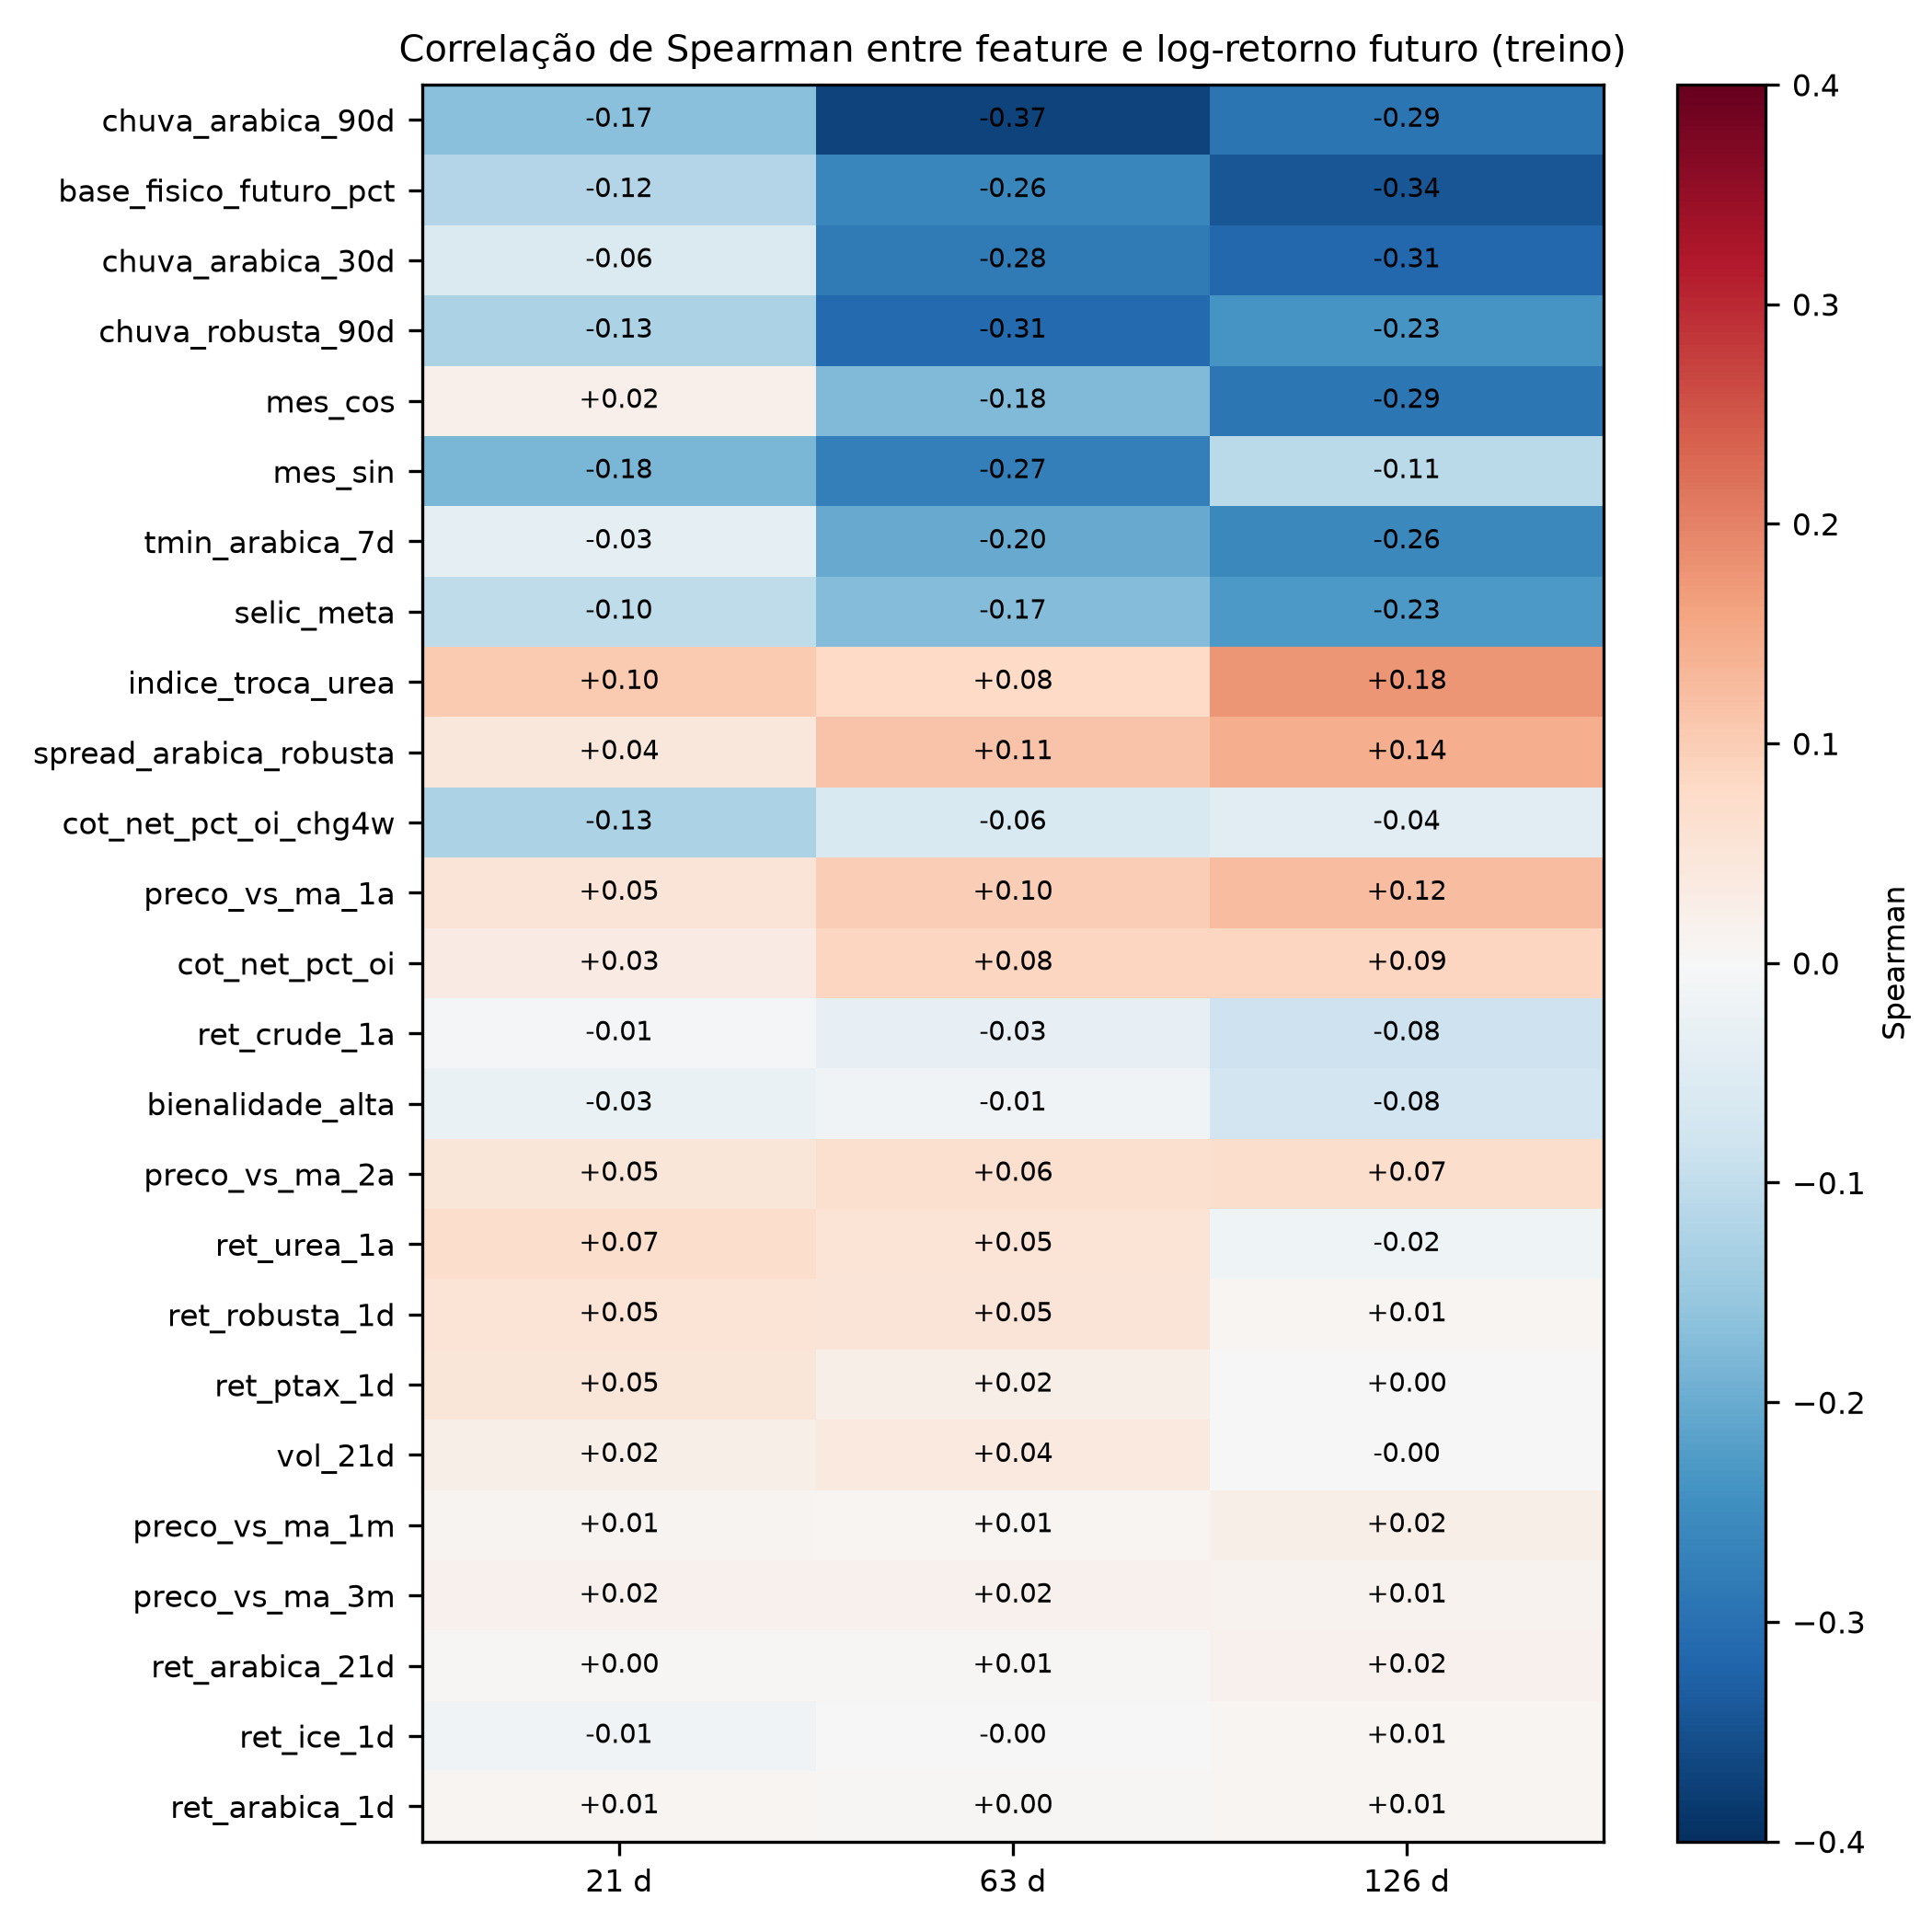
\includegraphics[width=0.95\textwidth]{imgs/10_corr_features_alvo.png}
	\fonte{Do autor (2026).}
\end{figure}

\begin{figure}[htb]
	\centering
	\caption{Matriz de correlação de Spearman entre as variáveis de entrada, no conjunto de treino.}\label{fig:matriz-corr}
	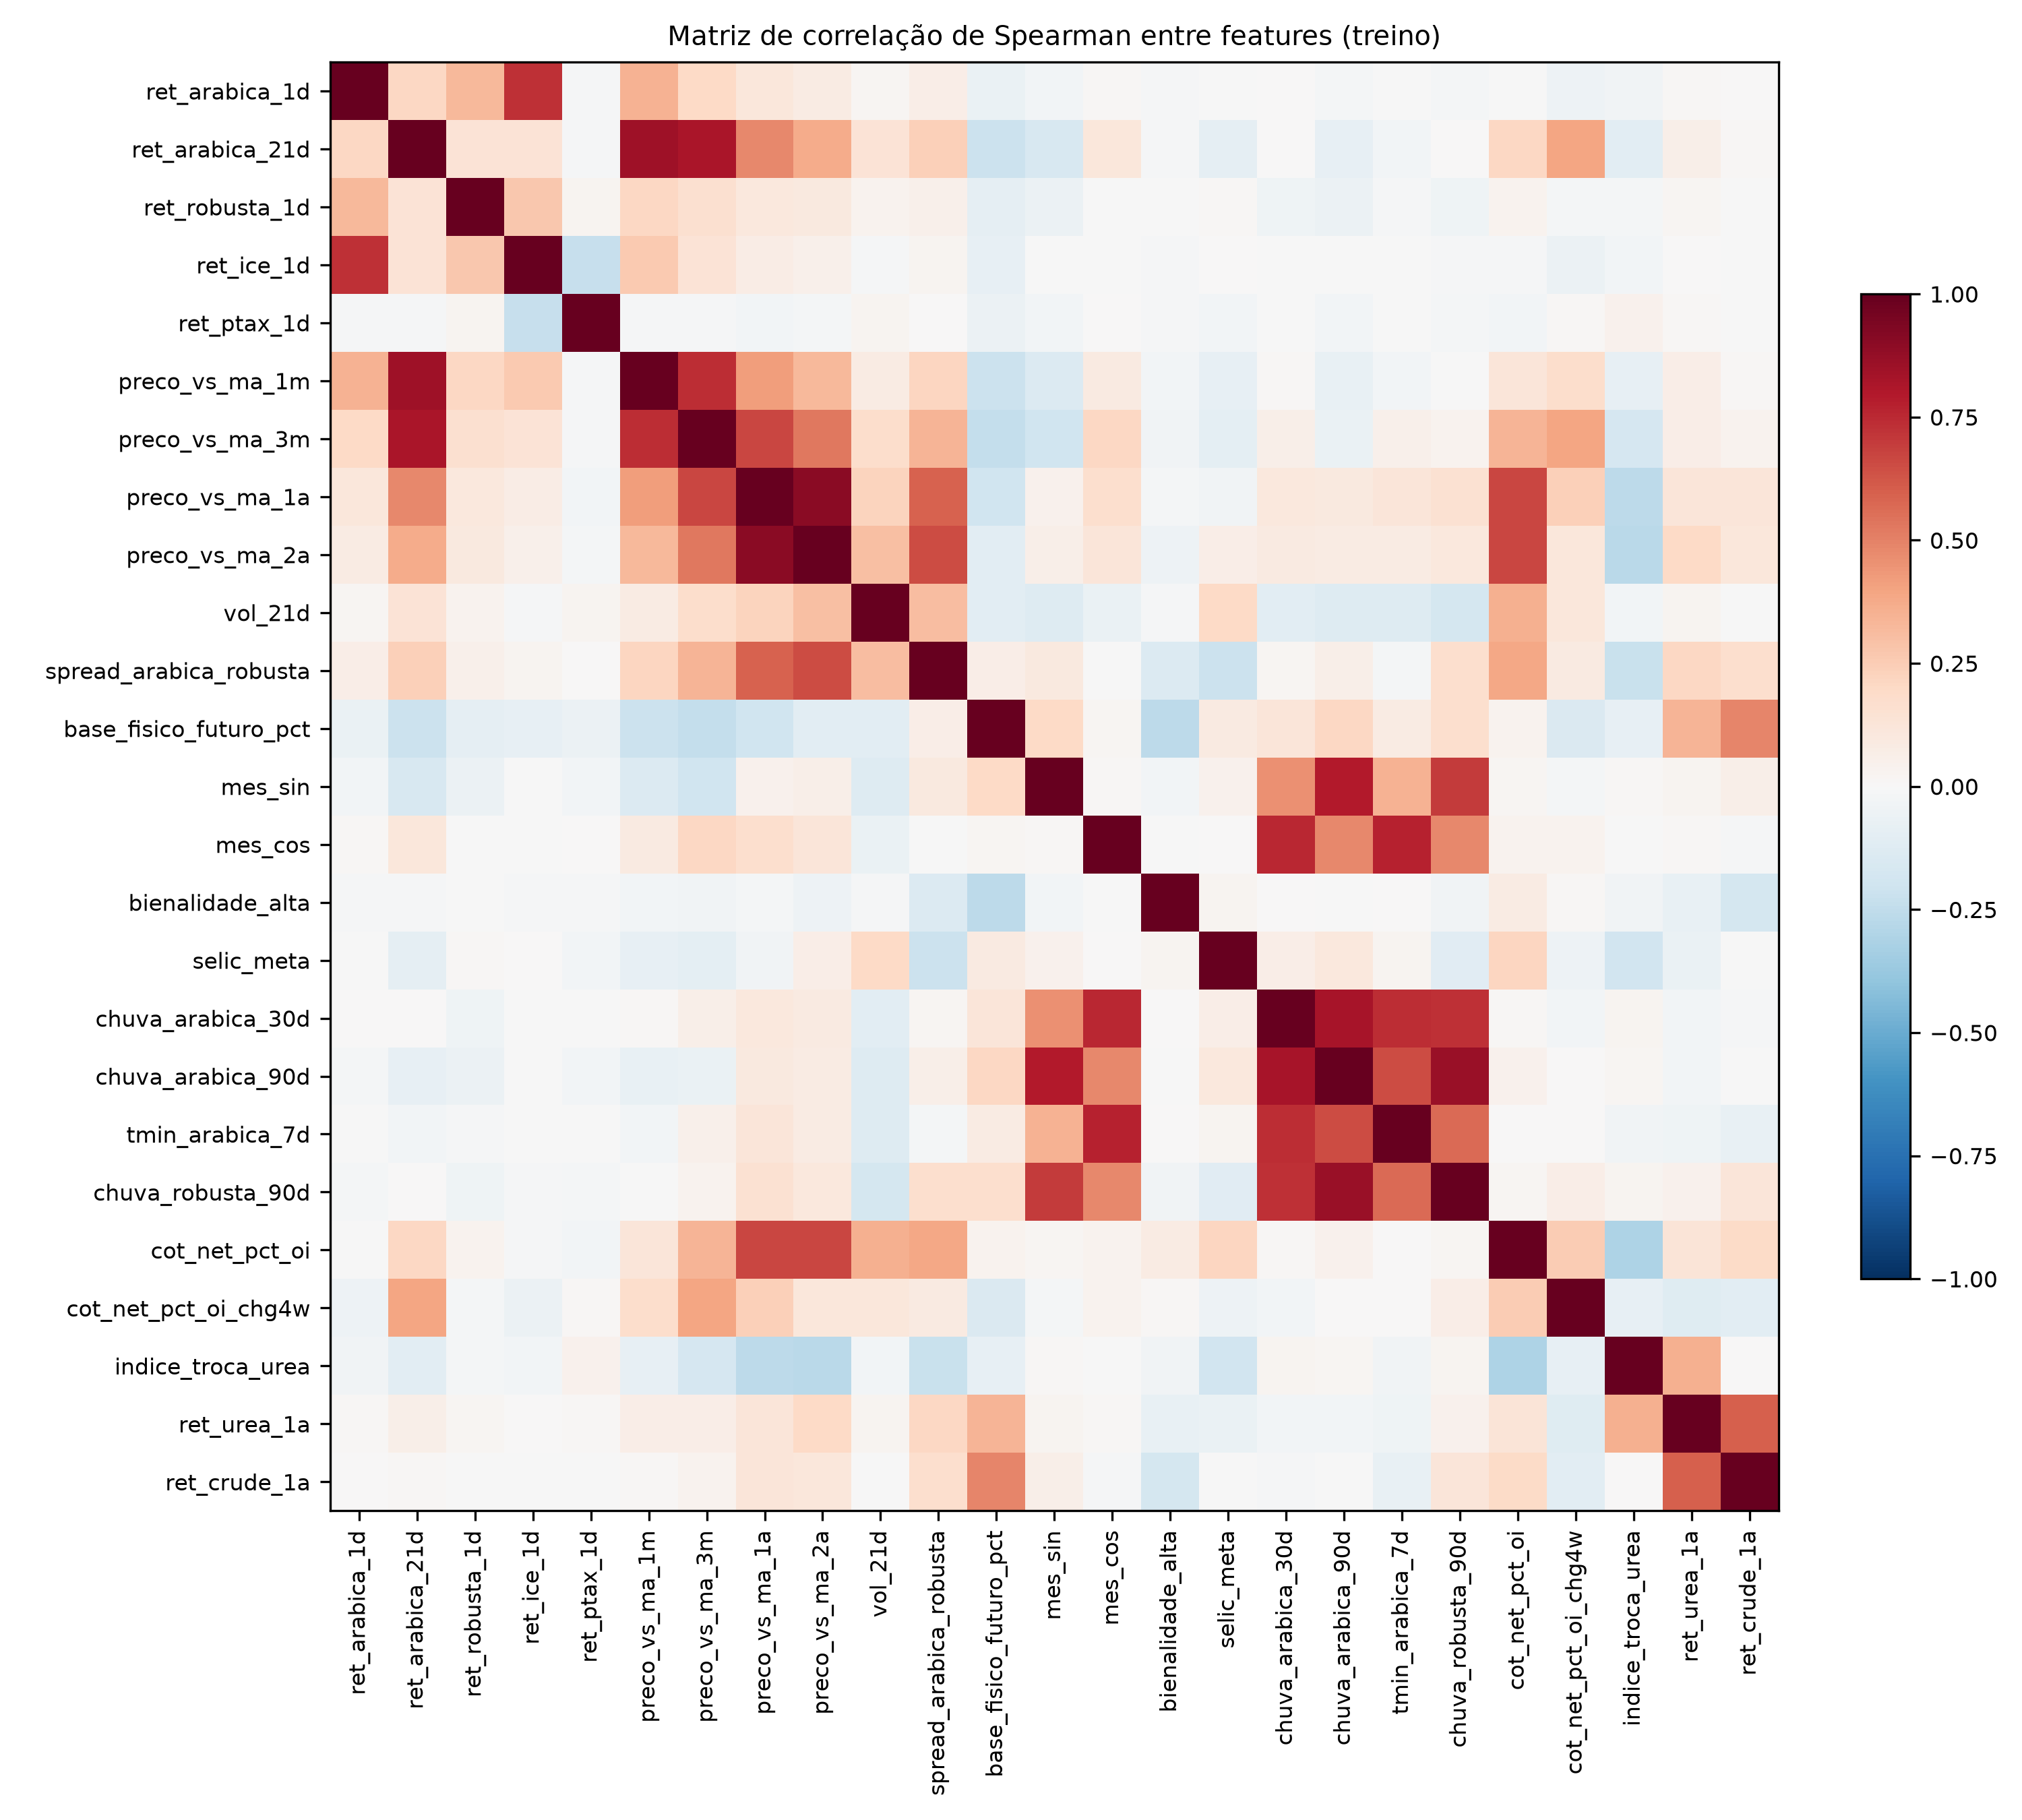
\includegraphics[width=0.95\textwidth]{imgs/11_matriz_corr_features.png}
	\fonte{Do autor (2026).}
\end{figure}

Três padrões orientaram as decisões seguintes. Primeiro, o sinal está nas variáveis de oferta, de base e de calendário, e cresce com o horizonte: o acumulado de chuva de 90 dias nas regiões de arábica tem correlação de $-0{,}37$ com o retorno de 63 dias, a base físico-futuro de $-0{,}34$ com o de 126 dias, o acumulado de 30 dias de $-0{,}31$ com o de 126 dias, a mínima de sete dias de $-0{,}26$ e a meta Selic de $-0{,}23$ no mesmo horizonte. O sinal negativo da chuva é o esperado: chuva abundante na floração melhora a expectativa da safra seguinte e o mercado a precifica para baixo. Segundo, as variáveis de curto prazo carregam pouco ou nenhum sinal: retornos diários, retorno de 21 dias, posição em relação às médias de um e três meses e volatilidade têm correlação inferior a $0{,}04$ em módulo em todos os horizontes. Terceiro, clima e calendário medem em parte a mesma coisa, a estação do ano: as correlações entre a codificação do mês e os acumulados de chuva e a mínima de temperatura ficam entre $0{,}7$ e $0{,}8$, e os acumulados de chuva de 90 dias das regiões de arábica e de robusta têm correlação $0{,}9$. Também são quase redundantes as razões com as médias de um e dois anos ($0{,}9$) e o retorno de 21 dias com a razão à média de um mês ($0{,}8$).

Nenhuma variável foi removida com base nessa análise. A rede recorrente tolera colinearidade entre entradas, o \textit{dropout} penaliza a dependência de uma única variável, e a contribuição de cada grupo é medida diretamente, por ablação e por importância por permutação, no \autoref{sec:resultados}. A colinearidade entre clima e calendário, porém, condiciona a leitura dessas medidas: ao remover um dos grupos, o outro pode compensá-lo em parte. A análise revelou ainda que o indicador de geada é constante igual a zero em toda a série, porque a reanálise ERA5 nunca registra temperatura mínima abaixo de 3\,$^{\circ}$C nos quatro pontos de grade escolhidos, nem mesmo em julho de 2021. A variável foi mantida entre as 26 entradas, onde é inerte após a normalização, e a consequência para a validade de construção é discutida no \autoref{sec:ameacas}.

\subsection{Partição temporal e normalização}

A partição é estritamente cronológica e usa o ano-safra, iniciado em julho, como unidade. O conjunto de teste cobre exatamente duas safras, porque a bienalidade define um ciclo de dois anos e uma única safra representaria apenas metade dele. A \autoref{tab:split} apresenta os cortes.

\begin{table}[htb]
	\centering
	\caption{Partição cronológica da base de dados.}\label{tab:split}
	\small
	\begin{tabular}{l L{3.3cm} L{2.6cm} r L{4.2cm}}
		\hline
		\textbf{Conjunto} & \textbf{Período} & \textbf{Safras} & \textbf{Amostras} & \textbf{Uso} \\ \hline
		Treino & 07/12/2005 a 30/06/2022 & 2005/06 a 2021/22 & 3\,940 & Pesos e normalizador \\
		Validação & 01/07/2022 a 30/06/2024 & 2022/23 e 2023/24 & 372 & Parada antecipada, dispersão residual, base sazonal \\
		Teste & 01/07/2024 a 31/08/2026 & 2024/25 e 2025/26 & 417 & \textit{Backtest} cego \\ \hline
	\end{tabular}
	\fonte{Do autor (2026).}
\end{table}

A janela de entrada de uma amostra pode cruzar a fronteira com o conjunto anterior, uma vez que se trata de histórico já conhecido na data da previsão. O alvo nunca cruza: as últimas 126 datas de cada conjunto são descartadas como origem de amostra, para que nenhum rótulo do treino seja calculado com preços da validação, nem rótulo da validação com preços do teste. Por esse motivo as amostras de validação terminam em dezembro de 2023 e as de teste em março de 2026.

A normalização usa um padronizador global ajustado exclusivamente no conjunto de treino e aplicado sem reajuste à validação e ao teste. A alternativa de normalizar em janelas deslizantes foi considerada e descartada porque as variáveis já são estacionárias por construção, o que torna o padronizador global suficiente e mais simples de auditar.

\section{Operacionalização da Ferramenta}\label{sec2:operacionalizacao}

O AgroVisible é organizado em dois módulos desacoplados. O módulo preditivo recebe a janela de variáveis e devolve a previsão central e a dispersão do log-retorno em cada horizonte. O módulo prescritivo recebe essa distribuição, os parâmetros econômicos do produtor e a curva de futuros, e devolve a política ótima. A interface entre os dois é apenas um vetor de médias e um vetor de desvios-padrão por horizonte, de forma que o módulo preditivo pode ser substituído por qualquer outro estimador sem alteração no motor de decisão.

\subsection{Módulo preditivo}

A rede é uma LSTM empilhada, implementada em Keras, com a arquitetura resumida no \autoref{qua:lstm}. Ela recebe uma janela de 63 dias úteis por 26 variáveis e produz três saídas treinadas em conjunto: o log-retorno em 21, 63 e 126 dias úteis,
\begin{equation}
	y_h(t) = \ln P(t+h) - \ln P(t), \qquad h \in \{21, 63, 126\},
\end{equation}
em que $P$ é o indicador CEPEA em R\$/sc. O preço projetado é reconstruído por $\hat{P}(t+h) = P(t)\,e^{\hat{y}_h(t)}$. A escolha de log-retornos como alvo, em vez do preço em nível, elimina a tendência da série e faz com que erros sejam comparáveis entre períodos de preço baixo e alto.

\begin{quadro}[htb]
	\centering
	\caption{Configuração do módulo preditivo.}\label{qua:lstm}
	\begin{tabular}{L{4cm} L{10cm}}
		\hline
		\textbf{Elemento} & \textbf{Configuração} \\ \hline
		Entrada & Janela de 63 dias úteis $\times$ 26 variáveis \\
		Camadas & LSTM(32, sequências) $\to$ Dropout 0,4 $\to$ LSTM(16) $\to$ Dropout 0,4 $\to$ Dense(32, ReLU) $\to$ Dense(3, linear) \\
		Saídas & Log-retorno em 21, 63 e 126 dias úteis \\
		Função de perda & Erro quadrático médio sobre os log-retornos \\
		Otimizador & Adam, taxa inicial $10^{-3}$, redução por patamar (fator 0,5, paciência 7) \\
		Treinamento & Até 100 épocas, lote 32, parada antecipada na perda de validação (paciência 15, restaura os melhores pesos); o modelo final parou na época 26 \\
		Seleção & Unidades e \textit{dropout} escolhidos por busca no conjunto de validação (\autoref{sec3:busca-hp}); janela, lote, taxa e paciências fixados a priori \\
		Reprodutibilidade & Semente 42; execução em CPU \\ \hline
	\end{tabular}
	\fonte{Do autor (2026).}
\end{quadro}

Além da previsão central, o módulo estima a incerteza da previsão pelo desvio-padrão dos resíduos $\hat{y}_h - y_h$ no conjunto de validação, um valor por horizonte. Esse desvio é o único canal pelo qual a qualidade da previsão chega ao motor de decisão: quanto maior o erro histórico da rede em um horizonte, mais largo é o cone de preços que o motor considera nesse horizonte.

\subsection{Busca de hiperparâmetros}\label{sec3:busca-hp}

A configuração inicial do módulo preditivo foi fixada a priori, antes de qualquer experimento: 64 unidades na primeira camada recorrente e 32 na segunda, \textit{dropout} 0,2, janela de 63 dias úteis, escolhida por cobrir um trimestre, igual ao horizonte intermediário, lote 32 e taxa de aprendizado $10^{-3}$. Para verificar se essa capacidade era adequada a uma amostra de 3\,940 janelas de treino, foi conduzida uma busca em duas etapas, sobre o conjunto de validação e sem uso do conjunto de teste para escolher.

Na primeira etapa, uma grade de doze configurações variou um fator por vez a partir da configuração inicial: unidades (32 e 128), \textit{dropout} (0 e 0,4), janela (21 e 126 dias), taxa de aprendizado ($3 \times 10^{-4}$ e $3 \times 10^{-3}$) e lote (64), além de duas candidatas enxutas com 32 unidades e \textit{dropout} 0,4, uma com janela de 63 e outra de 126 dias. Cada configuração foi treinada uma única vez, com semente 42 e o mesmo critério de parada antecipada, e comparada pelo RMSE em cada horizonte e pela média dos três horizontes na validação. O RMSE de treino foi registrado como indicador de sobreajuste: uma configuração que erra muito menos no treino do que na validação está memorizando a amostra.

Na segunda etapa, as três configurações mais promissoras, a inicial e as duas de 32 unidades com janela de 63 dias, foram retreinadas com cinco sementes (42 a 46) e avaliadas na validação e no teste, reportando média e desvio-padrão entre sementes ao lado dos métodos de referência. A escolha do modelo final foi feita pela média de validação; as métricas de teste dessa etapa servem apenas para confirmar que a ordem entre as candidatas não é um artefato do conjunto de validação. Os resultados da busca estão na \autoref{sec2:res-hp}, e a implicação de ter selecionado a arquitetura na validação é tratada como ameaça à validade interna no \autoref{sec:ameacas}.

\subsection{Módulo prescritivo}

O problema de comercialização é formulado como um processo de decisão de Markov de horizonte finito \cite{Puterman1994}, resolvido por indução retroativa sobre a equação de Bellman \cite{Bellman1957}.

\paragraph{Tempo e estado.} O tempo avança em passos mensais $k = 0, 1, \ldots, K$, com $K = 6$ (126 dias úteis), que é o horizonte máximo de previsão da rede. O estado é o par $(k, x)$, em que $x = \ln P$ é o logaritmo do preço físico em R\$/sc, discretizado em uma grade de 121 pontos centrada no preço da data de decisão.

\paragraph{Transição.} O log-preço evolui por incrementos gaussianos cuja média e variância vêm do módulo preditivo:
\begin{equation}
	x_{k+1} = x_k + \Delta\mu_k + \varepsilon_k, \qquad \varepsilon_k \sim \mathcal{N}(0, \Delta\sigma_k^2).
\end{equation}
A previsão central e o desvio residual dos três horizontes são interpolados linearmente para os sete passos mensais; a variância acumulada é forçada a ser não decrescente. A transição entre grades consecutivas é uma matriz gaussiana discretizada e normalizada por linha. Não há amostragem de cenários: a indução retroativa integra sobre toda a distribuição em cada passo.

\paragraph{Ações.} Em cada estado o produtor escolhe entre três ações:
\begin{alineas}
	\item \textbf{vender}: recebe $P_k (1-q)^k$ por saca, em que $q$ é a quebra técnica mensal, e encerra o processo;
	\item \textbf{armazenar}: paga o custo de armazenagem $c_{\text{arm}}$ do mês e segue exposto ao preço;
	\item \textbf{armazenar com \textit{hedge}} até o vencimento $m > k$: vende o contrato futuro de vencimento $m$ e armazena até lá, recebendo o preço travado $F_{k,m}(1 + b_m) - c_{\text{op}}$, sujeito apenas ao risco de base, em que $b_m$ é a base sazonal esperada no mês $m$ e $c_{\text{op}}$ o custo operacional de bolsa.
\end{alineas}

\paragraph{Função de valor.} A recompensa é a receita líquida por saca trazida a valor presente na data da decisão. O fator de desconto mensal deriva da meta Selic vigente, $\delta = (1 + i_{\text{Selic}})^{-1/12}$, e representa o custo de oportunidade do capital imobilizado no estoque. A função de valor é
\begin{equation}
	V_K(x) = P(x)\,(1-q)^K,
\end{equation}
\begin{equation}
	V_k(x) = \max\Big\{\, P(x)(1-q)^k,\;\; -c_{\text{arm}} + \delta\,\mathrm{CE}\big[V_{k+1}\big],\;\; \max_{m > k} H_{k,m}(x) \Big\}, \quad k < K,
	\label{eq:bellman}
\end{equation}
em que $H_{k,m}$ é o valor presente do \textit{hedge} até $m$ e $\mathrm{CE}[\cdot] = \mathbb{E}[\cdot] - \lambda\,\mathrm{DP}[\cdot]$ é o equivalente certo, com $\lambda \geq 0$ o parâmetro de aversão a risco do produtor. Com $\lambda = 0$ o produtor é neutro a risco e maximiza a receita esperada.

O custo operacional efetivo (COE) entra no motor como piso econômico da comercialização. Como o COE é um custo já incorrido na data da decisão, ele não altera a comparação marginal entre vender e armazenar em um dado estado; seu papel é outro: vender abaixo do COE configura descapitalização da empresa rural \cite{AgroSafety2026}, e a ferramenta sinaliza ao produtor a margem sobre o COE em cada nó do grafo e classifica o resultado esperado de cada ação nas faixas de lucro supernormal, lucro normal, resíduo financeiro, descapitalização ou falência, conforme a relação entre a receita esperada e as camadas de custo COE, COT e custo total médio. Adicionalmente, o motor oferece uma restrição opcional, desligada por padrão, que só permite a ação de vender em nós com preço igual ou superior a COE$\times$(1 + m), com m uma margem mínima configurável, enquanto houver horizonte; no último período a venda é forçada. O COE por safra é lido da série histórica de custos de produção da CONAB para o café arábica em Guaxupé, Minas Gerais, com a correspondência COE = custo variável, COT = custo operacional e custo total conforme a nomenclatura da planilha.

\paragraph{Parâmetros econômicos.} A \autoref{tab:parametros} lista os valores padrão. A armazenagem e a quebra técnica são referências de mercado de armazéns gerais; a Selic é lida da série do Banco Central na data da decisão; o custo operacional de bolsa segue material de capacitação em gestão de risco agrícola.

\begin{table}[htb]
	\centering
	\caption{Parâmetros econômicos padrão do módulo prescritivo.}\label{tab:parametros}
	\small
	\begin{tabular}{L{5cm} L{4.6cm} L{4.2cm}}
		\hline
		\textbf{Parâmetro} & \textbf{Valor padrão} & \textbf{Origem} \\ \hline
		Armazenagem $c_{\text{arm}}$ & 2,50 R\$/sc/mês & Referência de armazém geral \\
		Quebra técnica $q$ & 0,2 \%/mês & Referência de mercado \\
		Taxa de desconto & 10\,\% a.a. (Selic vigente na sensibilidade) & BCB, série 432 \\
		Custo operacional de bolsa $c_{\text{op}}$ & 10 R\$/sc & Material de capacitação \\
		COE por safra & 766 a 876 R\$/sc & CONAB, Guaxupé, MG \\
		Aversão a risco $\lambda$ & 0 & Parâmetro do usuário \\ \hline
	\end{tabular}
	\fonte{Do autor (2026).}
\end{table}

\paragraph{Grafo de decisão.} O objeto que o motor resolve é uma cadeia de Markov em camadas: sete camadas temporais com 121 nós de preço cada, e arestas de cada nó para todos os nós da camada seguinte, ponderadas pela transição gaussiana. A indução retroativa percorre esse grafo direcionado acíclico da última camada para a primeira, e o resultado é a ação ótima em cada nó, o gatilho de preço a partir do qual vender é ótimo em cada mês, e a distribuição de probabilidade do mês de venda. Para fins de apresentação ao produtor, uma árvore reduzida com três ramos por mês (quantis 10, 50 e 90 do cone de preços) é anotada com as ações lidas da política completa; essa árvore ilustra a política, mas não participa do cálculo.

\paragraph{Base e \textit{hedge}.} A base é definida em percentual do futuro convertido, $b = (P - F_{\text{R\$}}) / F_{\text{R\$}}$, em que $F_{\text{R\$}}$ é o \textit{Coffee C} convertido de centavos de dólar por libra-peso para reais por saca de 60 kg pela PTAX do dia. A modelagem em percentual, e não em reais, decorre da observação de que a base em reais escala com o nível de preço. A base esperada por mês do ano e o risco de base por horizonte (desvio-padrão da variação da base) são estimados de 2015 até o fim do conjunto de treino. O contrato ICE convertido é usado como \textit{proxy} do contrato ICF da B3, cuja série histórica não está disponível publicamente.

\paragraph{Operação em política rolante.} Em uso corrente, o sistema é executado a cada data de decisão com a janela de 63 dias úteis encerrada naquela data; a rede recebe apenas dados já observados e publicados até ela, respeitando as datas de disponibilidade descritas na \autoref{sec2:pipeline}. A previsão nova substitui a anterior, o horizonte de seis meses é recontado a partir da nova data e a política é resolvida de novo. Uma saca que foi armazenada no mês anterior é, portanto, reavaliada com a informação mais recente e vendida assim que a ação ótima do novo estado for vender, mesmo que a política do mês anterior previsse mantê-la por mais tempo. O produtor recebe, a cada mês, a ação do dia, o gatilho de venda por mês futuro e a distribuição de probabilidade do mês de venda. É esse mecanismo rolante que o \textit{backtest} e a simulação por safra reproduzem. Neste estudo a rede foi treinada uma única vez, com dados até junho de 2022, e não é retreinada entre decisões; a periodicidade de retreino em operação é uma decisão de implantação, discutida no \autoref{sec:discussao}.

\section{Protocolo de Avaliação}\label{sec2:protocolo}

\subsection{Avaliação preditiva (RQ1)}

A acurácia é medida no conjunto de validação e no conjunto de teste, por horizonte, com RMSE e MAE no espaço do log-retorno e MAPE no preço reconstruído, além da acurácia direcional (proporção de previsões com o sinal correto). Os métodos de referência são:
\begin{alineas}
	\item \textbf{passeio aleatório}: retorno previsto igual a zero em todos os horizontes;
	\item \textbf{curva de futuros com base sazonal}: retorno implícito $\ln\big[F_t\,(1 + b_{t+h}) / P_t\big]$, em que $F_t$ é o futuro convertido e $b_{t+h}$ a base sazonal esperada no mês de destino;
	\item \textbf{ARIMA} sobre o log-preço diário, com ordem $(p,d,q)$, $p,q \in \{0,1,2\}$, selecionada por AIC no conjunto de treino; parâmetros fixos, previsão recursiva a partir de cada data.
\end{alineas}

A seleção da arquitetura segue o protocolo da \autoref{sec3:busca-hp}: grade de doze configurações com semente única e verificação das candidatas com cinco sementes. Como referência para a variabilidade de treino, o modelo final é treinado com cinco sementes distintas, e toda diferença entre modelos menor que o desvio-padrão entre sementes é tratada como empate.

A contribuição das variáveis exógenas é medida por três instrumentos complementares. A correlação de Spearman com o alvo, calculada antes do treinamento (\autoref{sec3:eda}), indica onde há sinal nos dados. A importância por permutação mede, no modelo final treinado, o aumento do RMSE de validação quando os valores de uma variável são embaralhados dentro da janela de entrada, na média de três permutações; ela indica de quais variáveis a rede efetivamente depende. A ablação, por fim, retreina a rede com a mesma configuração removendo, um por vez, cada um de seis grupos de variáveis (retornos e médias móveis; mercado; calendário e Selic; clima; fundos; insumos), com três sementes por configuração, e registra a variação relativa do RMSE médio por horizonte; ela indica o que se perde quando o grupo não está disponível.

\subsection{Avaliação prescritiva (RQ2)}

O \textit{backtest} simula um produtor que, em cada data de decisão, dispõe de uma saca colhida e deve decidir o que fazer com ela ao longo dos seis meses seguintes. As datas de decisão são mensais, de 1º de julho de 2024 a 3 de fevereiro de 2026, totalizando 20 decisões distribuídas em duas safras. Em cada data o motor é resolvido com a previsão e a Selic daquela data, sem acesso a qualquer informação posterior, e a política é executada contra os preços efetivamente observados. A receita de cada estratégia é a receita líquida por saca em valor presente na data da decisão, com a mesma contabilidade de armazenagem, quebra e desconto para todas.

As estratégias comparadas são:
\begin{alineas}
	\item \textbf{venda imediata}: vende na data da decisão e aplica o valor à taxa de desconto até o fim do horizonte. Como todas as receitas são trazidas a valor presente pela mesma taxa, isso equivale a comparar cada estratégia com a alternativa de vender hoje e investir o resultado à Selic;
	\item \textbf{venda parcelada}: vende um sexto da saca em cada um dos seis meses;
	\item \textbf{média móvel de três meses}: vende quando o preço cruza acima da média móvel de 63 dias, ou no fim do horizonte;
	\item \textbf{meta de margem sobre o COE}: vende quando o preço alcança 130 \% do COE, ou no fim do horizonte;
	\item \textbf{\textit{hedge} de seis meses}: vende o futuro na data da decisão e entrega no fim do horizonte;
	\item \textbf{AgroVisible}: executa a política ótima resolvida pela \autoref{eq:bellman};
	\item \textbf{oráculo}: vende no melhor mês do horizonte com conhecimento perfeito do futuro; é o limite superior, não uma estratégia viável.
\end{alineas}

As duas primeiras são as heurísticas nomeadas na RQ2. As demais foram acrescentadas por serem praticadas por produtores e cooperativas e por isolarem componentes específicos do AgroVisible: a média móvel testa uma regra técnica simples; a meta de margem testa uma regra de custo; o \textit{hedge} fixo testa o instrumento de proteção isoladamente. O oráculo permite expressar o ganho de cada estratégia como fração do ganho máximo disponível.

O mesmo protocolo é aplicado às 18 datas mensais do período de validação, de julho de 2022 a dezembro de 2023, que contém regime de queda de preços, ampliando a amostra para 38 decisões em quatro safras. Nesse período a dispersão residual e a parada antecipada da rede foram calibradas com os próprios dados, o que é declarado como viés favorável leve ao interpretar os resultados. A significância das diferenças de receita é avaliada por diferença pareada por data, com intervalo de confiança de 95\,\% por \textit{bootstrap} de 10\,000 reamostragens e teste de Wilcoxon pareado.

\paragraph{Simulação por safra.} O \textit{backtest} mensal avalia vinte decisões independentes, cada uma com uma saca recém-colhida, o que mede a qualidade média da política, mas não reproduz a situação do produtor, que colhe uma vez por ano. Por isso o mesmo motor é avaliado em uma segunda forma: uma saca colhida no primeiro dia útil de julho de cada ano-safra, de 2022 a 2025, com até doze meses para ser vendida. A política é rolante, como descrito na \autoref{sec2:operacionalizacao}: a cada mês o motor é resolvido de novo com a previsão daquela data e o prazo restante, e a saca é vendida no primeiro mês em que a ação ótima for vender. Como o horizonte de doze meses excede o alcance de 126 dias da rede, além desse ponto a deriva prevista é mantida no último valor e a incerteza cresce com a raiz do tempo, como em um passeio aleatório, extrapolação conservadora que só afeta os meses finais de uma trajetória que é reavaliada mensalmente. As mesmas estratégias de referência são simuladas no horizonte de doze meses e a receita é expressa em valor presente na data da colheita. As safras 2024/25 e 2025/26 são cegas; 2022/23 e 2023/24 pertencem ao período de validação, com o viés já declarado.

\subsection{Análise de sensibilidade (RQ3)}

A sensibilidade é avaliada repetindo o \textit{backtest} completo sob uma grade de parâmetros e registrando a receita líquida média e a frequência de decisões de armazenar. A grade cobre a aversão a risco ($\lambda \in \{0; 0{,}25; 0{,}5; 1\}$), o custo de armazenagem ($\{1{,}5; 2{,}5; 5{,}0\}$ R\$/sc/mês), a taxa de desconto (8, 10, 12, 13,25 e 15\,\% a.a., além da Selic vigente em cada data) e o choque de base (deslocamento de $\pm 5$ pontos percentuais na base esperada e duplicação do risco de base). O caso base adota taxa de desconto de 10\,\% a.a., valor próximo à média da Selic na amostra.

\subsection{Ambiente de execução}

Todos os experimentos foram executados em Python 3.13, com TensorFlow 2.21 e Keras 3.15 para a rede neural, NumPy 2.5 e SciPy 1.18 para o motor de decisão, pandas 3.0 para o alinhamento dos dados, scikit-learn 1.9 para a normalização e statsmodels 0.15 para o ARIMA, em um computador pessoal com Windows 11, em CPU, sem aceleração por GPU, e com semente fixa. O código está organizado em cinco cadernos numerados (coleta, variáveis, previsão, decisão e simulação por safra) e em módulos reutilizáveis, de modo que cada tabela e figura dos capítulos seguintes pode ser regenerada a partir dos dados brutos. O código, os dados e os resultados intermediários estão versionados em um repositório Git.

\chapter{\MakeUppercase{Resultados Experimentais}}\label{sec:resultados}

Este capítulo apresenta os resultados na ordem das questões de pesquisa. A \autoref{sec2:res-rq1} avalia o componente preditivo; a \autoref{sec2:res-rq2} apresenta o \textit{backtest} financeiro; a \autoref{sec2:res-rq3} apresenta a análise de sensibilidade. Todos os experimentos foram executados em 23 de setembro de 2026 com a configuração descrita no \autoref{sec:configuracao}. O caso base do motor prescritivo usa armazenagem de 2,50 R\$/sc/mês, quebra técnica de 0,2 \%/mês, taxa de desconto de 10 \% a.a., neutralidade a risco ($\lambda = 0$) e \textit{hedge} habilitado; a Selic vigente em cada data é tratada como um dos cenários de sensibilidade.

\section{Resultados para a RQ1: acurácia preditiva}\label{sec2:res-rq1}

\subsection{LSTM contra os métodos de referência}

A \autoref{tab:rq1-metricas} apresenta as métricas da rede e dos três métodos de referência nos conjuntos de validação e de teste, por horizonte. As métricas de erro estão no espaço do log-retorno; o MAPE é o erro percentual equivalente no preço reconstruído.

\begin{table}[htb]
	\centering
	\caption{Acurácia por horizonte nos conjuntos de validação (372 amostras) e teste (417 amostras). RMSE e MAE em log-retorno; MAPE em \% do preço; direção em \% de acertos de sinal.}\label{tab:rq1-metricas}
	\footnotesize
	\setlength{\tabcolsep}{3.5pt}
	\begin{tabular}{l l r r r r r r r}
		\hline
		\textbf{Conjunto} & \textbf{Horiz.} & \multicolumn{4}{c}{\textbf{LSTM}} & \multicolumn{3}{c}{\textbf{RMSE das referências}} \\
		& & RMSE & MAE & MAPE & Direção & Passeio aleat. & ARIMA(1,1,2) & Curva futuros \\ \hline
		Validação & 21 d  & 0,112 & 0,081 & 8,7  & 55,6 & \textbf{0,091} & \textbf{0,090} & 0,107 \\
		          & 63 d  & 0,194 & 0,158 & 17,6 & 60,8 & 0,177 & 0,177 & \textbf{0,156} \\
		          & 126 d & \textbf{0,185} & 0,152 & 16,8 & 77,2 & 0,236 & 0,236 & 0,193 \\ \hline
		Teste     & 21 d  & 0,147 & 0,112 & 10,6 & 58,3 & \textbf{0,120} & \textbf{0,119} & 0,130 \\
		          & 63 d  & \textbf{0,213} & 0,150 & 13,9 & 71,5 & 0,233 & 0,233 & 0,227 \\
		          & 126 d & \textbf{0,267} & 0,192 & 16,9 & 79,1 & 0,321 & 0,321 & 0,309 \\ \hline
	\end{tabular}
	\fonte{Do autor (2026).}
\end{table}

Três padrões emergem. Primeiro, no horizonte de 21 dias a LSTM perde para o passeio aleatório e para o ARIMA nos dois conjuntos: no curto prazo, a melhor previsão do log-retorno é zero, e qualquer modelo que tente prever direção paga em variância. Segundo, o ARIMA é indistinguível do passeio aleatório em todos os horizontes, com RMSE igual até a terceira casa decimal e acerto direcional próximo de 50 \%, o que confirma que a série diária de log-preço é quase integrada e que o passeio aleatório é a referência estatística adequada. Terceiro, a vantagem da LSTM cresce com o horizonte: em 126 dias ela vence todas as referências nos dois conjuntos, com acerto direcional de 77 \% na validação e 79 \% no teste.

A curva de futuros ajustada pela base sazonal é a referência mais exigente. Na validação ela supera a LSTM em 21 e 63 dias e empata em 126. No teste, período de volatilidade recorde, a curva perde poder preditivo (acerto direcional de 42 a 61 \%) e a LSTM passa a vencê-la em 63 e 126 dias. Em termos de erro absoluto, todas as abordagens pioram do conjunto de validação para o de teste, reflexo do regime de preços sem precedente no período.

A \autoref{fig:previsto-realizado} mostra o previsto contra o realizado por horizonte no conjunto de teste e evidencia a principal deficiência do modelo: a compressão das previsões em direção a zero. As previsões raramente ultrapassam $\pm 0{,}2$ em log-retorno, enquanto os retornos realizados de 126 dias chegaram a $+0{,}57$ na alta do segundo semestre de 2024. A rede acerta a direção, mas subestima a magnitude dos movimentos extremos.

\begin{figure}[htb]
	\centering
	\caption{Log-retorno previsto contra realizado por horizonte no conjunto de teste.}\label{fig:previsto-realizado}
	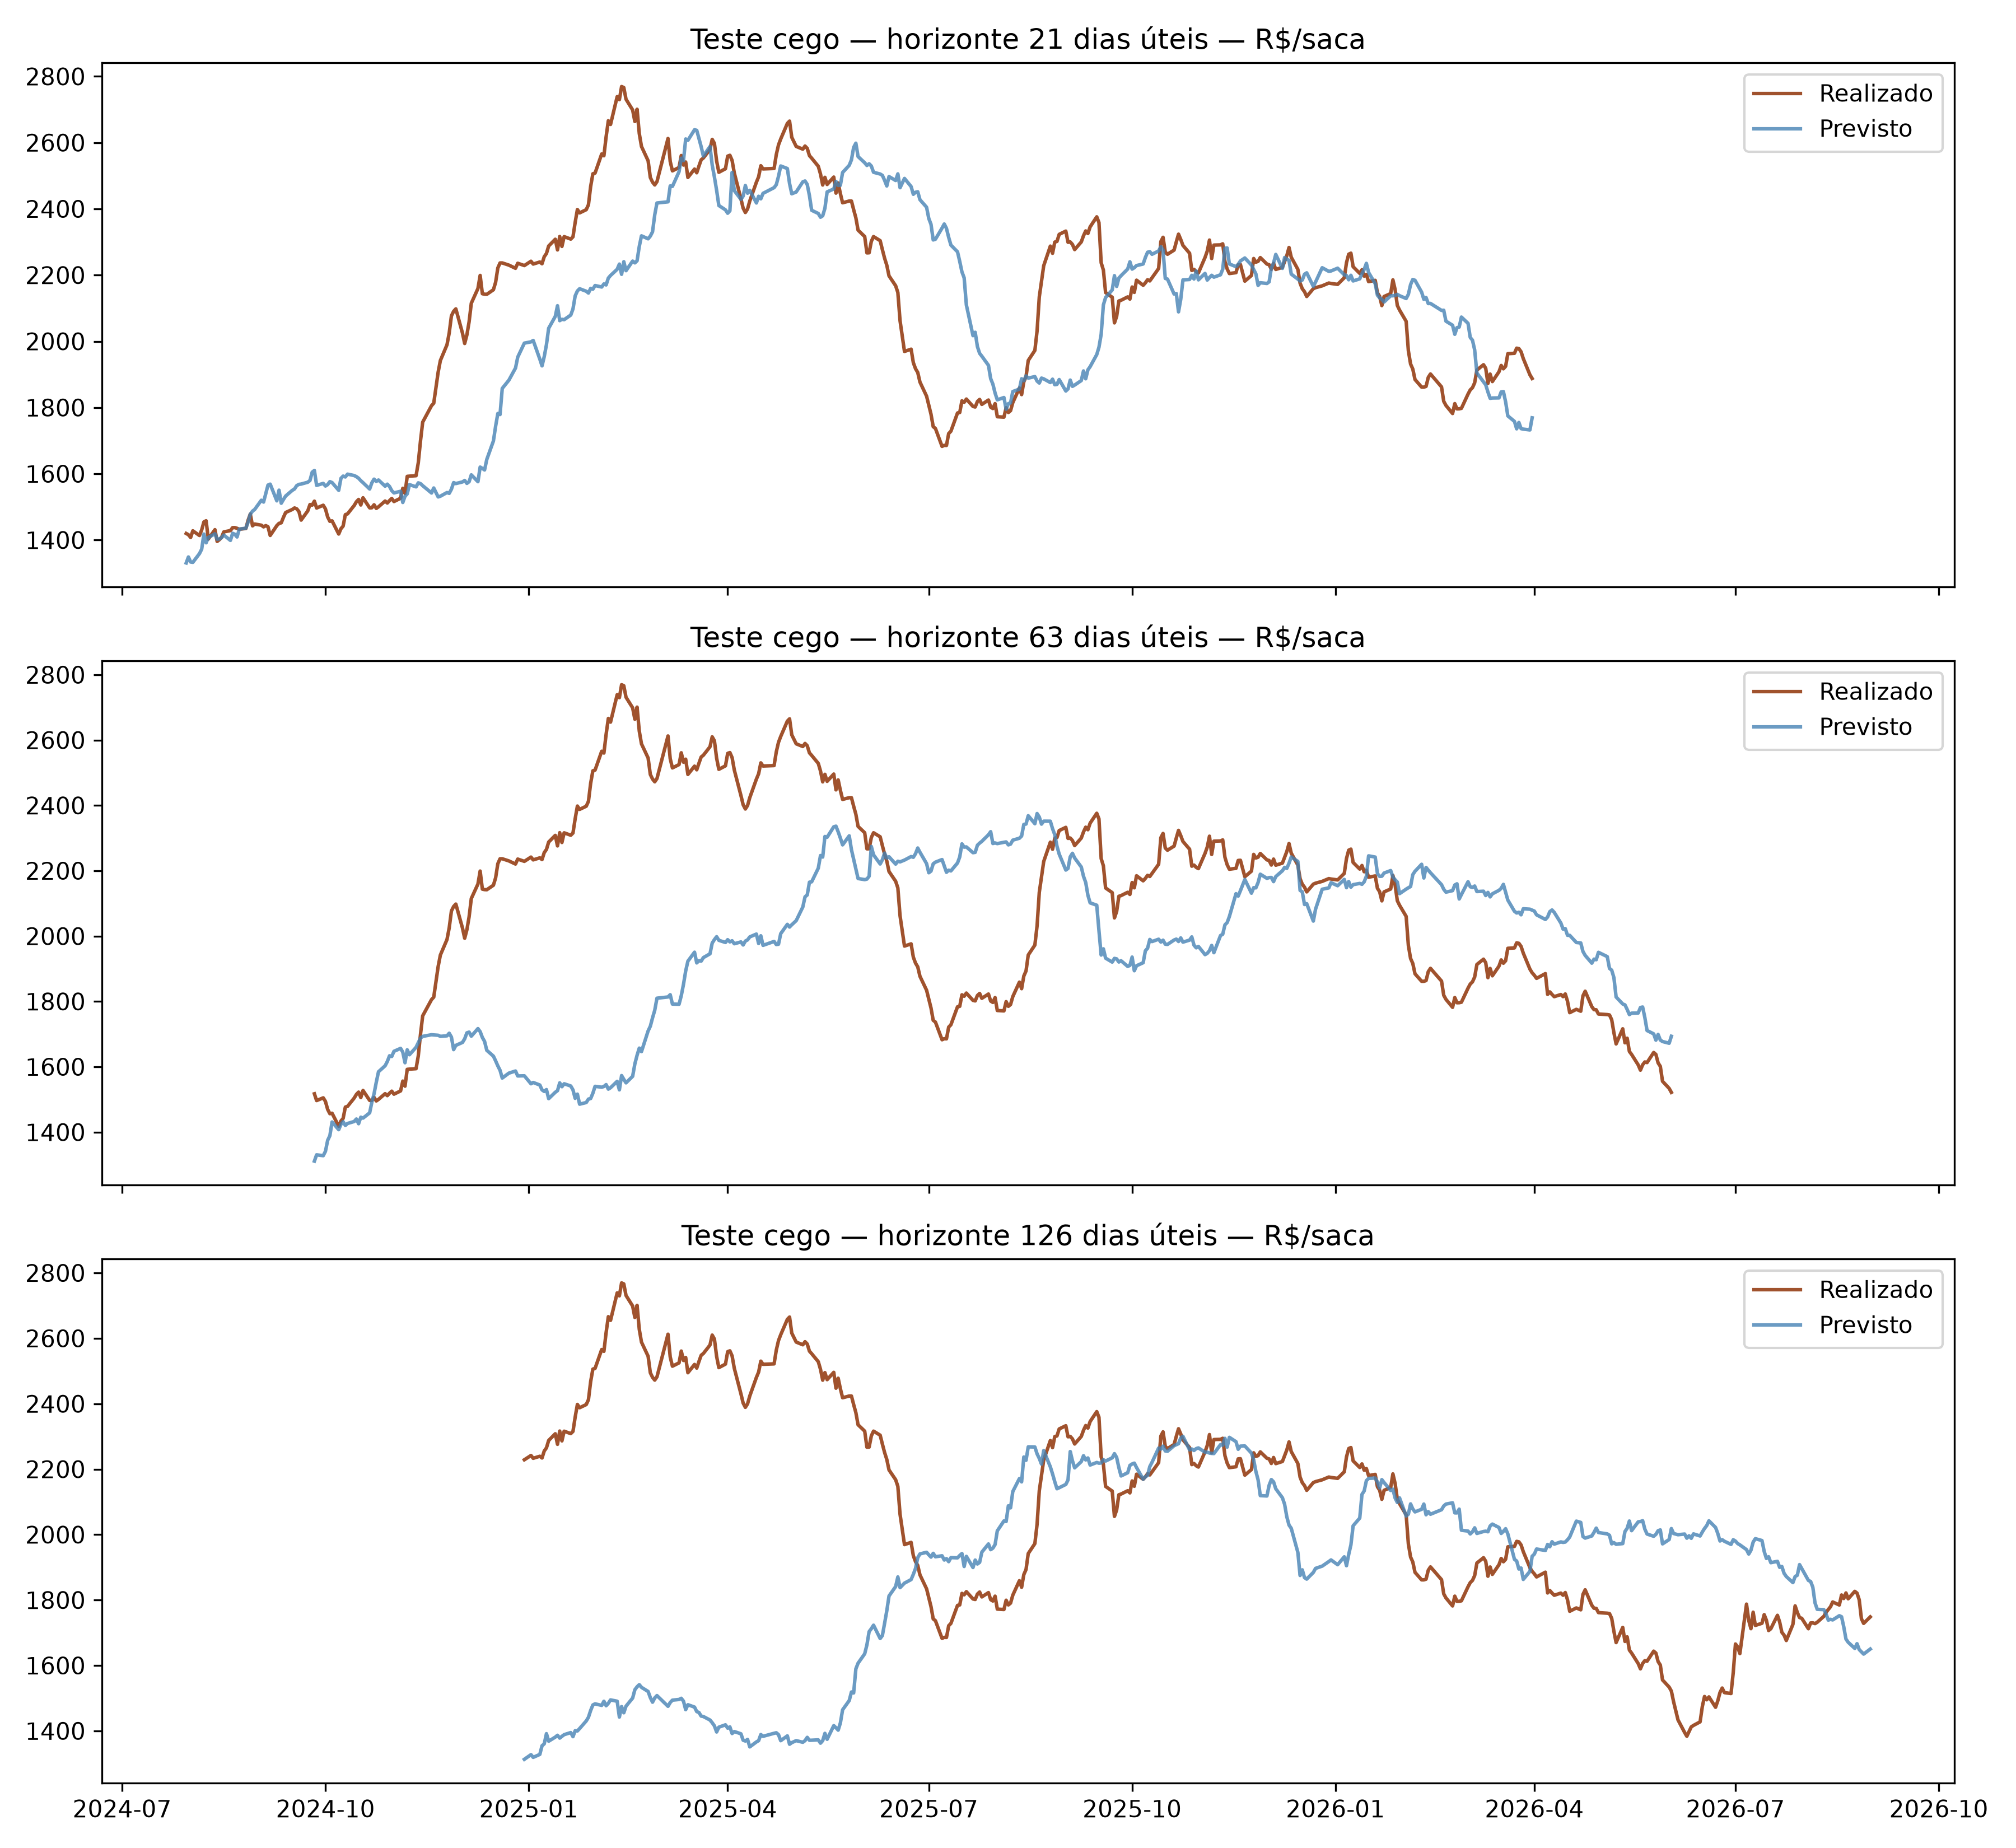
\includegraphics[width=\textwidth]{imgs/03_previsto_realizado_teste.png}
	\fonte{Do autor (2026).}
\end{figure}

\subsection{Variabilidade entre inicializações}

Antes de interpretar diferenças entre modelos é preciso conhecer a variabilidade do próprio treino. O modelo completo foi treinado com cinco sementes distintas; a \autoref{tab:rq1-seeds} resume o resultado na validação.

\begin{table}[htb]
	\centering
	\caption{Variabilidade do modelo completo entre cinco sementes (validação).}\label{tab:rq1-seeds}
	\begin{tabular}{l r r r}
		\hline
		\textbf{Métrica} & \textbf{Média} & \textbf{Desvio} & \textbf{Semente 42 (modelo final)} \\ \hline
		RMSE 21 d  & 0,114 & 0,008 & 0,112 \\
		RMSE 63 d  & 0,188 & 0,017 & 0,194 \\
		RMSE 126 d & 0,192 & 0,024 & 0,185 \\
		Direção 21 d (\%)  & 56,9 & 4,0 & 55,6 \\
		Direção 63 d (\%)  & 61,5 & 6,3 & 60,8 \\
		Direção 126 d (\%) & 74,1 & 8,2 & 77,2 \\ \hline
	\end{tabular}
	\fonte{Do autor (2026).}
\end{table}

O modelo final está dentro de um desvio-padrão da média em todas as métricas: não é o melhor nem o pior sorteio. A vantagem da curva de futuros sobre a LSTM na validação, de 0,008 em 21 dias e 0,032 em 63 dias, é da ordem de um desvio no primeiro caso e de quase dois no segundo. A diferença em 63 dias é, portanto, robusta à inicialização; a de 21 dias, não.

\subsection{Estudo de ablação}

Cada um dos seis grupos de variáveis foi removido por vez, e a rede foi retreinada com três sementes por configuração. A \autoref{tab:rq1-ablacao} apresenta a variação relativa do RMSE médio em relação ao modelo completo; valores positivos indicam que remover o grupo piorou o erro.

\begin{table}[htb]
	\centering
	\caption{Ablação por grupo de variáveis: variação relativa do RMSE médio de três sementes em relação ao modelo completo (validação). Positivo indica piora ao remover o grupo.}\label{tab:rq1-ablacao}
	\footnotesize
	\setlength{\tabcolsep}{4pt}
	\begin{tabular}{l r r r r}
		\hline
		\textbf{Grupo removido} & \textbf{$\Delta$ 21 d} & \textbf{$\Delta$ 63 d} & \textbf{$\Delta$ 126 d} & \textbf{Dir. 126 d} \\ \hline
		Nenhum (completo)          & ---     & ---    & ---     & 71,3 \% \\
		(a) Retornos e médias móveis & $-$10,1 \% & $-$6,9 \% & $-$10,0 \% & 77,4 \% \\
		(b) Mercado (vol., spread, base) & $-$6,7 \% & $-$8,3 \% & $+$10,4 \% & 59,5 \% \\
		(c) Calendário e Selic     & $+$3,9 \%  & $-$3,1 \% & $+$11,7 \% & 66,8 \% \\
		(d) Clima                  & $+$3,5 \%  & $+$6,1 \% & $-$9,4 \%  & 73,2 \% \\
		(e) Fundos (COT)           & $+$1,4 \%  & $-$6,5 \% & $-$12,4 \% & 75,8 \% \\
		(f) Insumos                & $+$7,2 \%  & $-$7,0 \% & $-$11,4 \% & 83,9 \% \\ \hline
	\end{tabular}
	\fonte{Do autor (2026).}
\end{table}

O desvio entre sementes dentro de cada configuração é de 2 a 5 \% do RMSE em 21 e 63 dias e de cerca de 11 \% em 126 dias, de modo que apenas efeitos acima dessa ordem merecem interpretação. Com esse critério, a ablação sustenta quatro conclusões.

\begin{alineas}
	\item Os grupos de \textbf{mercado} e de \textbf{calendário e Selic} são os que carregam sinal de longo prazo: removê-los piora o RMSE de 126 dias em 10 a 12 \% e derruba o acerto direcional nesse horizonte de 71 \% para 59 \% e 67 \%.
	\item O \textbf{clima} contribui nos horizontes de 21 e 63 dias, com piora de 3 a 6 \% ao ser removido, mas não em 126 dias.
	\item Remover \textbf{retornos e médias móveis}, \textbf{fundos} ou \textbf{insumos} melhora o erro de 126 dias em 10 a 12 \%. Esses grupos, no modelo completo, adicionam mais ruído que informação no horizonte longo.
	\item A ablação não sustenta a hipótese de que todas as variáveis exógenas contribuem para a acurácia. Sustenta que um subconjunto (mercado, calendário, Selic e clima) é essencial e que uma versão enxuta do modelo é candidata natural para reduzir o sobreajuste discutido no \autoref{sec:discussao}.
\end{alineas}

\section{Resultados para a RQ2: ganho financeiro da prescrição}\label{sec2:res-rq2}

\subsection{Backtest no teste cego}

A \autoref{tab:rq2-teste} apresenta a receita líquida média por saca, em valor presente, das sete estratégias nas 20 datas de decisão do teste cego, separadas por safra. A \autoref{fig:receita-por-data} mostra a receita de cada estratégia em cada data.

\begin{table}[htb]
	\centering
	\caption{Receita líquida média por saca (R\$, valor presente) no teste cego, por safra.}\label{tab:rq2-teste}
	\footnotesize
	\setlength{\tabcolsep}{3.5pt}
	\begin{tabular}{l r r r r r r r r}
		\hline
		\textbf{Safra} & \textbf{n} & \textbf{Imed.} & \textbf{Parc.} & \textbf{M. móvel} & \textbf{Meta COE} & \textbf{Hedge} & \textbf{AgroVis.} & \textbf{Oráculo} \\ \hline
		2024/25 & 12 & 1\,999 & \textbf{2\,057} & 1\,996 & 1\,999 & 1\,805 & 2\,003 & 2\,418 \\
		2025/26 & 8  & 2\,072 & 1\,919 & 1\,963 & 2\,072 & 2\,076 & \textbf{2\,199} & 2\,202 \\
		Total   & 20 & 2\,028 & 2\,001 & 1\,983 & 2\,028 & 1\,913 & \textbf{2\,081} & 2\,331 \\ \hline
	\end{tabular}
	\fonte{Do autor (2026).}
\end{table}

\begin{figure}[htb]
	\centering
	\caption{Receita líquida por data de decisão no teste cego, todas as estratégias.}\label{fig:receita-por-data}
	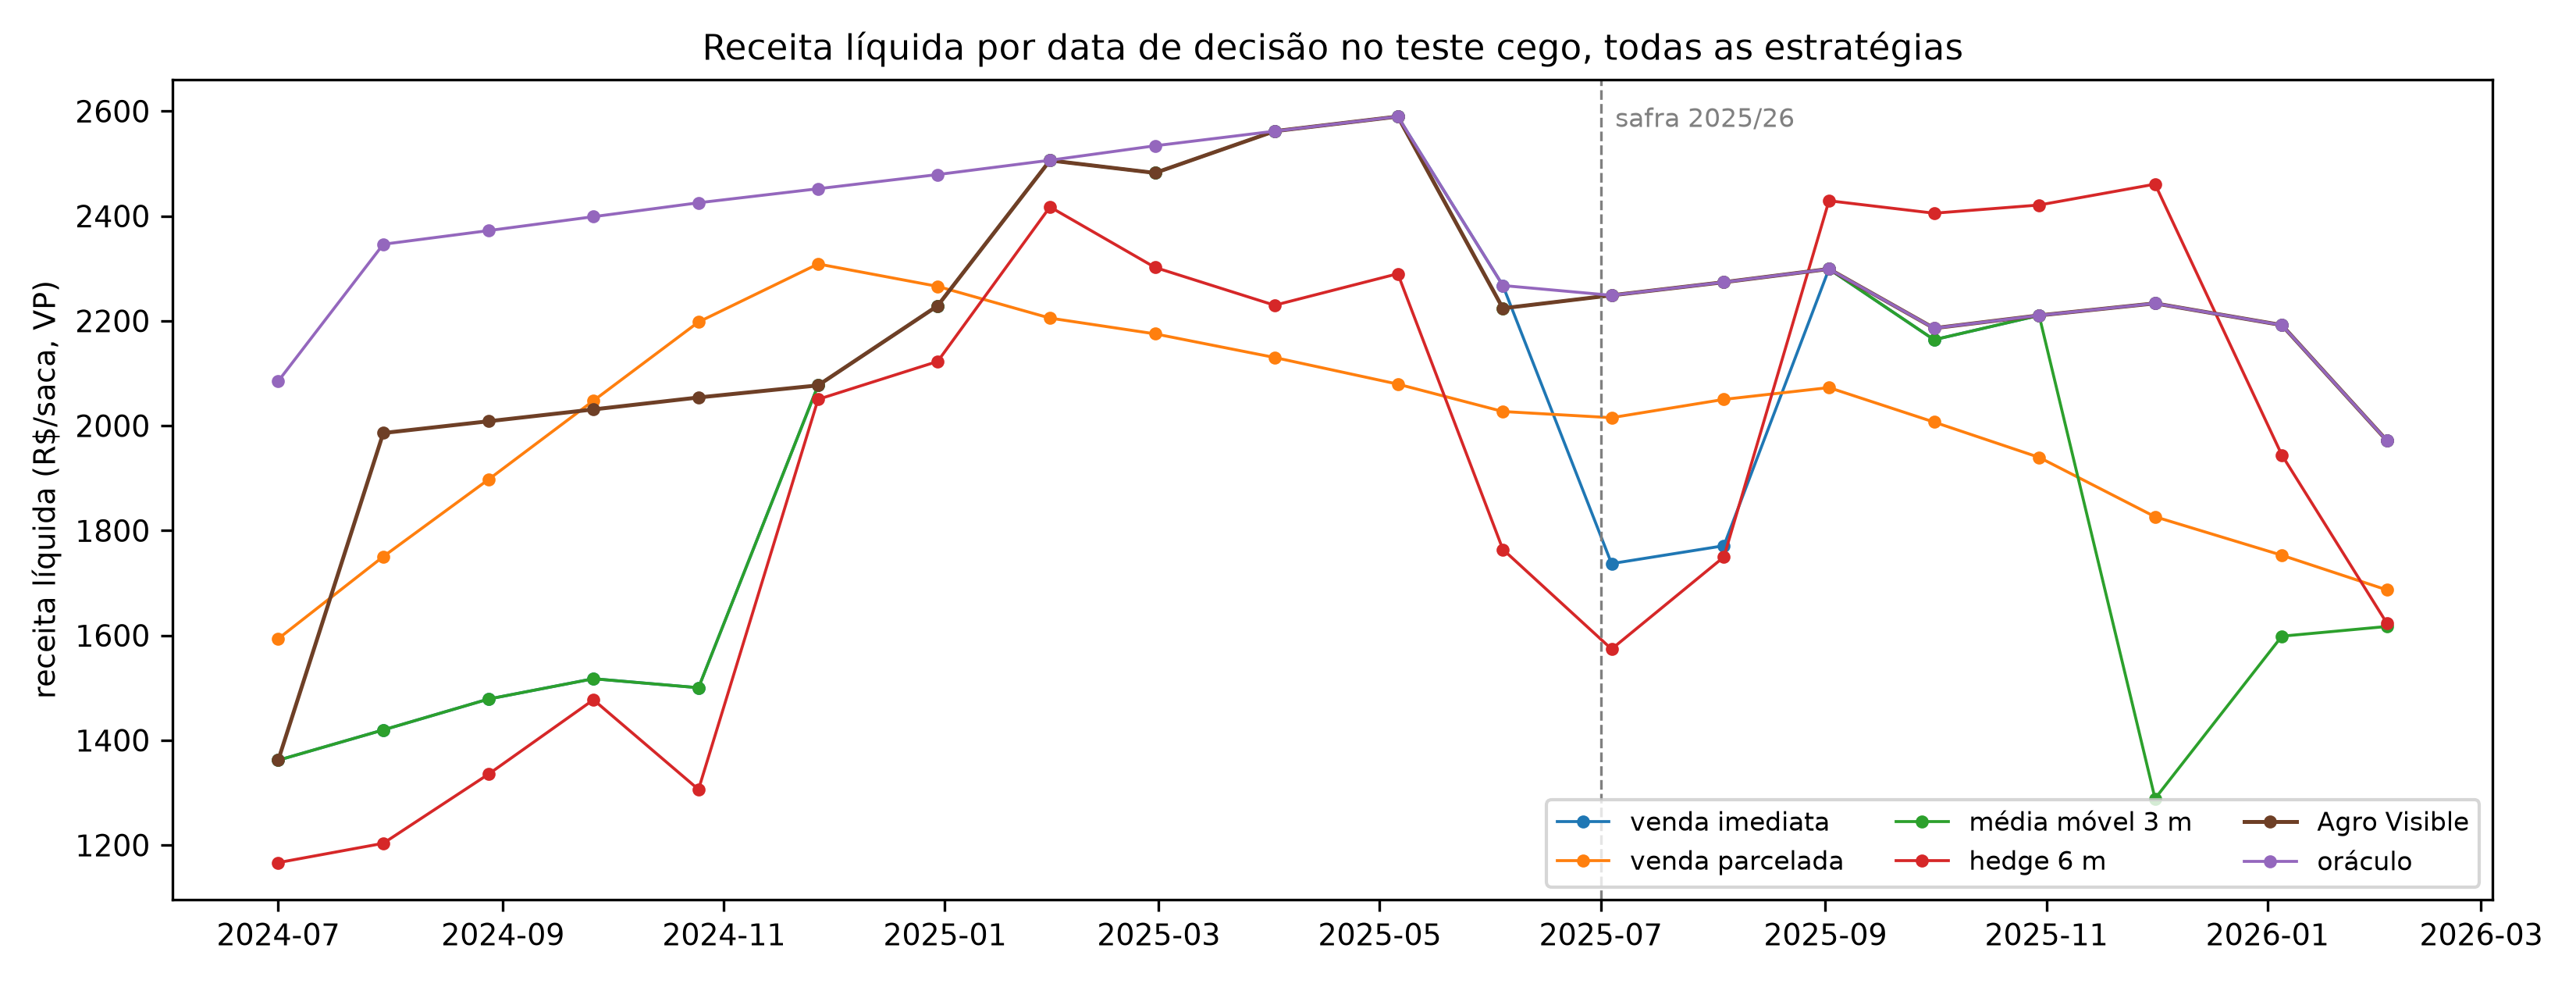
\includegraphics[width=\textwidth]{imgs/07_receita_por_data_teste.png}
	\fonte{Do autor (2026).}
\end{figure}

No agregado das 20 datas, o AgroVisible obteve 2\,081 R\$/sc contra 2\,028 da venda imediata, ganho de 2,6 \%, e contra 2\,001 da venda parcelada, ganho de 4,0 \%. As duas safras, porém, contam histórias opostas.

Na safra 2024/25 o café subiu de 1\,362 R\$/sc em julho de 2024 para mais de 2\,500 em janeiro de 2025, uma alta de 84 \% em seis meses. A estratégia vencedora foi a venda parcelada, que diluiu a venda ao longo da alta sem precisar prevê-la. O AgroVisible armazenou em julho e agosto de 2024, mas vendeu após um ou dois meses com ganhos de 4 \% e 1 \%, e vendeu imediatamente de setembro a dezembro porque a previsão de 21 dias era negativa em todas essas datas, enquanto o retorno realizado de 126 dias foi superior a 50 \%. O modelo não enxergou a alta persistente, e a compressão das previsões para zero fez o motor abandonar o estoque cedo. O resultado ficou praticamente igual ao da venda imediata.

Na safra 2025/26 ocorreu o oposto. Em julho e agosto de 2025, com o preço em torno de 1\,750 R\$/sc após uma queda de 30 \%, a rede previu recuperação, o motor armazenou por dois meses e um mês, respectivamente, e a receita foi 29 \% e 28 \% superior à venda imediata, capturando 100 \% do ganho do oráculo nessas datas. No platô alto que se seguiu, vender imediatamente era ótimo e foi o que o motor fez. A safra fechou em 2\,199 R\$/sc contra 2\,072 da venda imediata, a três reais do oráculo.

O \textit{hedge} de seis meses foi a pior estratégia no teste, com perda de 5,7 \% contra a venda imediata, porque o mercado esteve em \textit{backwardation} durante quase todo o período: vender o futuro travava um preço abaixo do físico. A meta de margem sobre o COE coincidiu com a venda imediata em todas as datas, pois o preço nunca esteve abaixo de 1,3 vez o COE. O motor nunca escolheu a ação de \textit{hedge} no \textit{backtest}, e a receita do AgroVisible com e sem essa ação é idêntica no teste.

\subsection{Ampliação da amostra ao período de validação}

Vinte decisões em duas safras de alta histórica constituem uma amostra pequena e atípica. O mesmo protocolo foi aplicado às 18 datas de decisão do período de validação, de julho de 2022 a dezembro de 2023, que inclui uma queda de 40 \% no preço. Nessas duas safras a dispersão residual e a parada antecipada da rede foram calibradas com os próprios dados, o que introduz um viés favorável leve à LSTM; as estatísticas de base já eram estimadas apenas no treino. A \autoref{tab:rq2-4safras} apresenta o resultado por safra e o consolidado de 38 datas.

\begin{table}[htb]
	\centering
	\caption{Receita líquida média por saca (R\$, valor presente) nas quatro safras. As safras 2022/23 e 2023/24 pertencem ao período de validação.}\label{tab:rq2-4safras}
	\footnotesize
	\setlength{\tabcolsep}{3.5pt}
	\begin{tabular}{l r r r r r r r r}
		\hline
		\textbf{Safra} & \textbf{n} & \textbf{Imed.} & \textbf{Parc.} & \textbf{M. móvel} & \textbf{Meta COE} & \textbf{Hedge} & \textbf{AgroVis.} & \textbf{Oráculo} \\ \hline
		2022/23 & 12 & \textbf{1\,139} & 992 & 1\,101 & \textbf{1\,139} & 1\,051 & 1\,106 & 1\,160 \\
		2023/24 & 6  & 853 & 919 & 859 & 922 & 758 & \textbf{958} & 1\,026 \\
		2024/25 & 12 & 1\,999 & \textbf{2\,057} & 1\,996 & 1\,999 & 1\,805 & 2\,003 & 2\,418 \\
		2025/26 & 8  & 2\,072 & 1\,919 & 1\,963 & 2\,072 & 2\,076 & \textbf{2\,199} & 2\,202 \\ \hline
		Total   & 38 & 1\,562 & 1\,512 & 1\,527 & 1\,573 & 1\,459 & \textbf{1\,596} & 1\,755 \\
		Ganho s/ imediata & & --- & $-$1,6\,\% & $-$1,7\,\% & $+$1,3\,\% & $-$7,7\,\% & $+$2,7\,\% & $+$14,0\,\% \\
		Captura oráculo & & 90,0\,\% & 86,5\,\% & 87,9\,\% & 91,1\,\% & 83,3\,\% & 91,9\,\% & 100\,\% \\ \hline
	\end{tabular}
	\fonte{Do autor (2026).}
\end{table}

Na safra 2022/23, de queda, o AgroVisible perdeu 3 \% para a venda imediata. Duas decisões em maio e junho de 2023 explicam quase toda a perda: a rede previu alta, o motor armazenou até o fim do horizonte e o preço caiu 20 \%, com perdas de 25 \% e 28 \% nessas datas. Na safra 2023/24, de recuperação a partir de um fundo, o motor armazenou em todas as datas e venceu todas as heurísticas, com ganho de 12 \% sobre a venda imediata.

No consolidado de quatro safras e dois regimes, o AgroVisible foi a única estratégia a superar a venda imediata em todos os agregados, com ganho de 2,7 \% e captura de 91,9 \% do valor do oráculo. A venda parcelada, que venceu na safra de alta, perdeu 1,6 \% no consolidado, porque carrega estoque durante as quedas. A \autoref{tab:rq2-oraculo} mostra a fração do ganho disponível capturada por cada estratégia nas datas em que o oráculo superava a venda imediata em mais de 1 \%, isto é, nas datas em que havia algo a ganhar armazenando.

\begin{table}[htb]
	\centering
	\caption{Fração do ganho do oráculo capturada, (estratégia $-$ imediata)/(oráculo $-$ imediata), média nas datas em que armazenar era vantajoso.}\label{tab:rq2-oraculo}
	\begin{tabular}{l r r}
		\hline
		\textbf{Estratégia} & \textbf{Teste (n = 11)} & \textbf{Quatro safras (n = 21)} \\ \hline
		Venda parcelada & $-$79,0 \% & $-$52,1 \% \\
		Média móvel 3 m & 18,2 \% & 28,3 \% \\
		Meta de margem COE & 0,0 \% & 15,1 \% \\
		Hedge 6 m & 51,7 \% & $-$22,7 \% \\
		AgroVisible & 19,0 \% & \textbf{47,4 \%} \\ \hline
	\end{tabular}
	\fonte{Do autor (2026).}
\end{table}

\subsection{Significância estatística}

A \autoref{tab:rq2-estatistica} apresenta a diferença pareada por data entre o AgroVisible e as duas heurísticas nomeadas na RQ2, com intervalo de confiança de 95 \% por \textit{bootstrap} de 10\,000 reamostragens e p-valor do teste de Wilcoxon pareado.

\begin{table}[htb]
	\centering
	\caption{Diferença pareada de receita por data (R\$/sc) entre o AgroVisible e as heurísticas.}\label{tab:rq2-estatistica}
	\footnotesize
	\setlength{\tabcolsep}{3.5pt}
	\begin{tabular}{l r l r r r r}
		\hline
		\textbf{Amostra} & \textbf{n} & \textbf{Comparação} & \textbf{Média} & \textbf{IC 95 \%} & \textbf{p (Wilcoxon)} & \textbf{Datas positivas} \\ \hline
		Teste & 20 & vs. imediata  & 52,8 & [$-$0,1; 128,6] & 0,271 & 20 \% \\
		Teste & 20 & vs. parcelada & 79,8 & [$-$76,0; 221,5] & 0,294 & 65 \% \\
		Quatro safras & 38 & vs. imediata  & 34,0 & [$-$6,8; 79,9] & 0,066 & 34 \% \\
		Quatro safras & 38 & vs. parcelada & 84,0 & [$-$3,1; 163,2] & \textbf{0,018} & 71 \% \\ \hline
	\end{tabular}
	\fonte{Do autor (2026).}
\end{table}

No teste isolado nenhuma diferença é significativa ao nível de 5 \%, o que era esperado com 20 observações e desvio-padrão da diferença de 156 R\$/sc. Com as 38 datas, a vantagem sobre a venda parcelada torna-se significativa ($p = 0{,}018$) e a vantagem sobre a venda imediata fica na margem ($p = 0{,}066$), com intervalo de confiança que inclui o zero por pouco. A baixa fração de datas positivas contra a venda imediata (34 \%) decorre da própria estrutura da política: na maioria das datas o motor vende imediatamente e a diferença é zero. O ganho concentra-se em poucas decisões de armazenar com retorno elevado, o que torna a média positiva mas a mediana nula, e é isso que o teste de Wilcoxon penaliza.

\subsection{Anatomia das decisões}

A \autoref{fig:gatilho} ilustra a saída do motor para a data de 31 de agosto de 2026, a mais recente disponível: para cada mês futuro, o preço a partir do qual vender é ótimo. Nos dois primeiros meses o gatilho está acima de 3\,000 R\$/sc, ou seja, a política é armazenar em quase qualquer cenário; do terceiro mês em diante o gatilho cai abaixo do preço corrente e a venda passa a ser recomendada assim que o preço previsto se estabiliza. Essa forma de política, armazenar enquanto a deriva prevista supera o custo de carregamento e vender quando ela se esgota, é a regra que o produtor recebe da ferramenta, e não uma única data de venda.

\begin{figure}[htb]
	\centering
	\caption{Gatilho de venda por mês para a decisão de 31 de agosto de 2026: preço a partir do qual vender é ótimo, contra o preço previsto.}\label{fig:gatilho}
	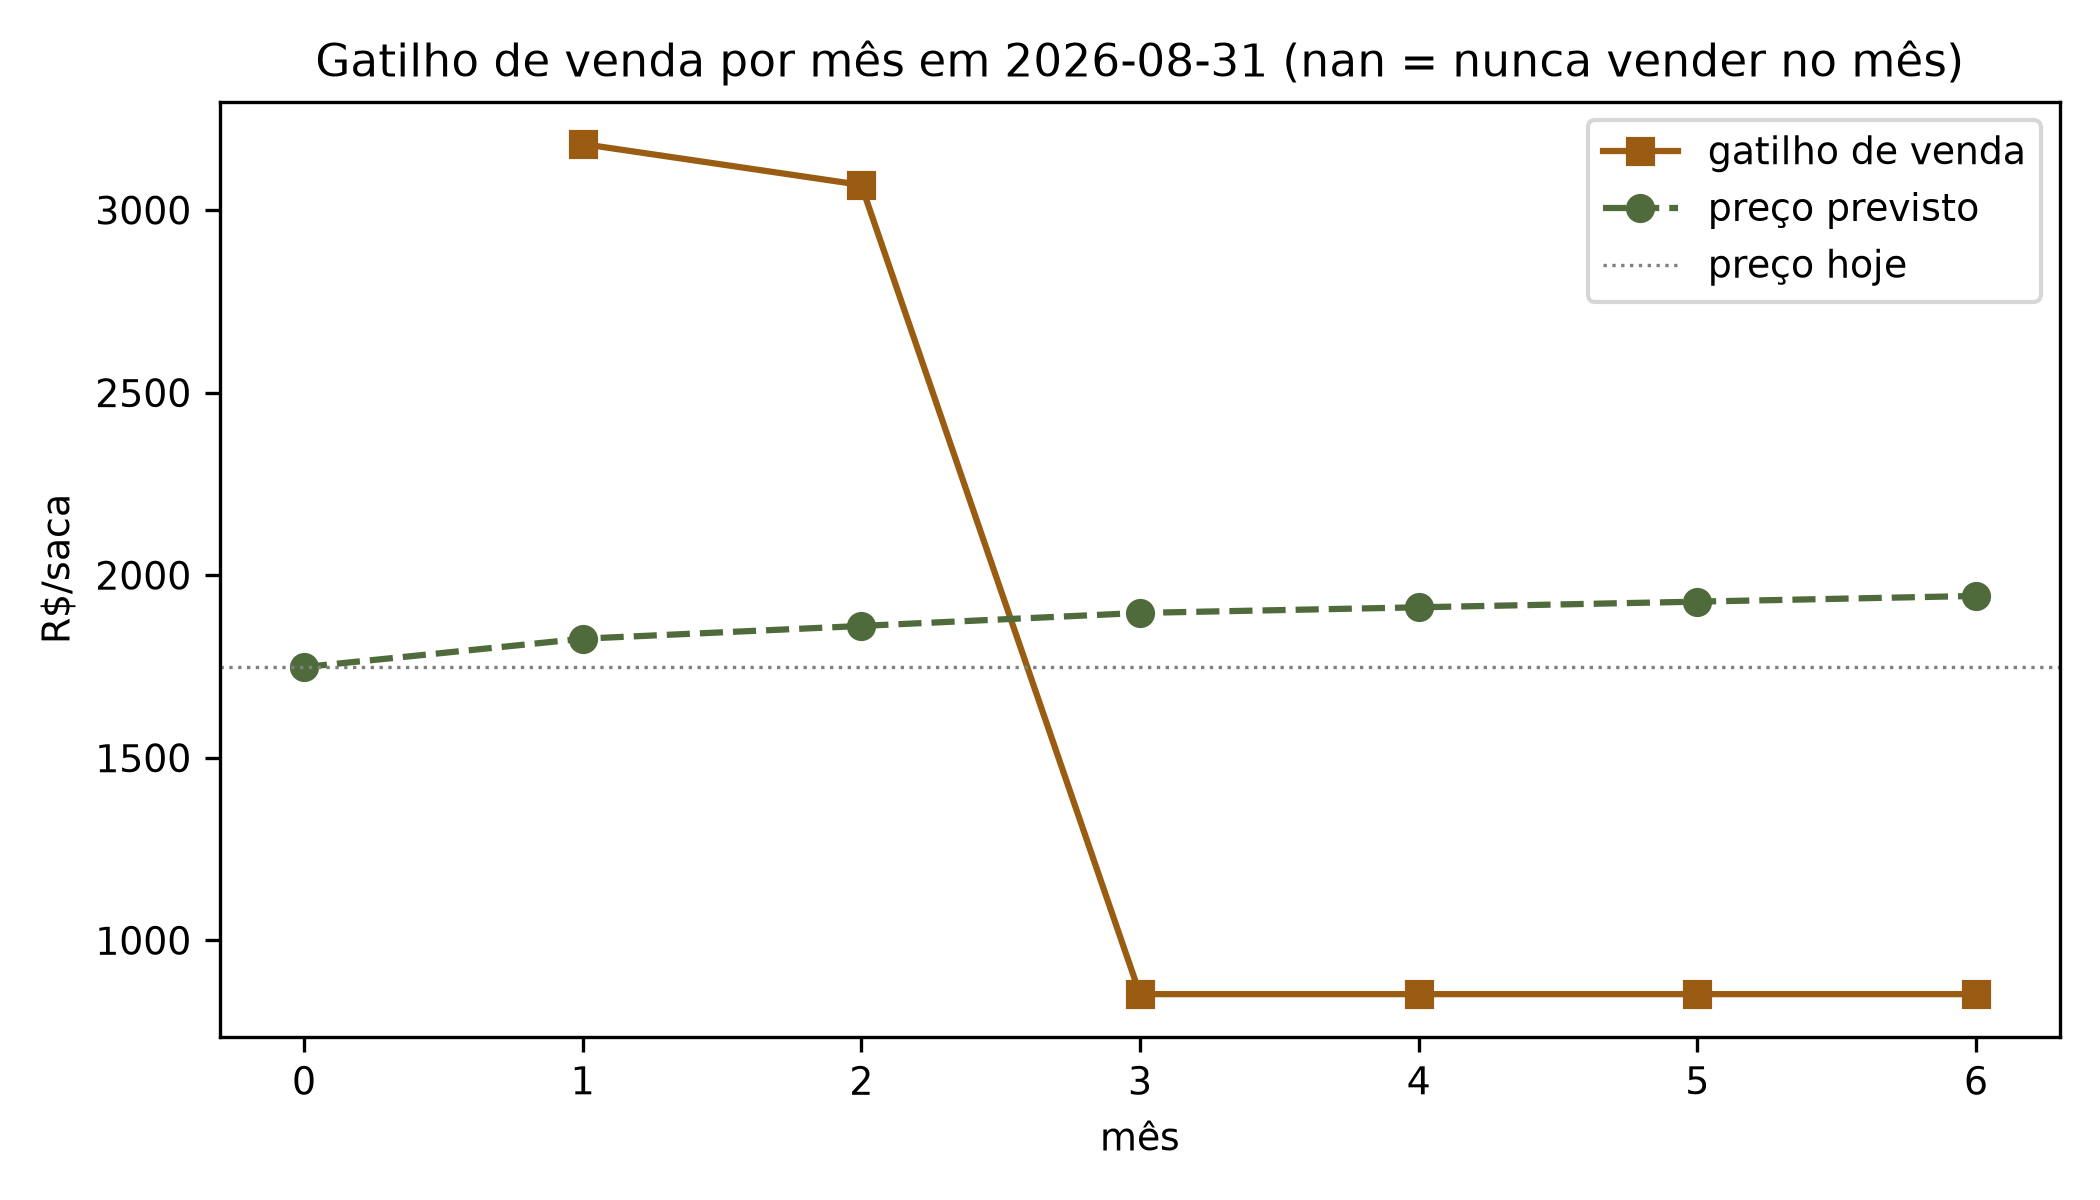
\includegraphics[width=0.85\textwidth]{imgs/06_gatilho_venda_por_mes.png}
	\fonte{Do autor (2026).}
\end{figure}

A decomposição por data das 38 decisões mostra que os quatro maiores ganhos (julho e agosto de 2025, julho e outubro de 2023) vieram de previsões de alta de 21 dias corretas em direção, e que as duas maiores perdas (maio e junho de 2023) vieram de previsões de alta erradas em datas de queda forte. Em cinco das 38 datas o motor armazenou e a venda imediata teria sido melhor; em treze, armazenou e ganhou; nas vinte restantes vendeu de imediato. O ganho médio positivo vem, portanto, de uma assimetria: quando o motor acerta a recuperação a partir de um fundo, o ganho é de 10 a 30 \%; quando erra, a perda média é menor, porque a política rolante revende o estoque assim que a previsão do mês seguinte deixa de justificar o carregamento.

\subsection{O custo operacional efetivo no motor}

O COE real por safra foi obtido da série histórica de custos de produção da CONAB para o café arábica em Guaxupé, Minas Gerais: 766, 714, 784 e 876 R\$/sc para as safras de 2022 a 2025. O valor provisório de 700 R\$/sc estava dentro da faixa. Com esses valores, a margem mínima observada sobre o COE no teste foi de 74 \%, e a restrição de não vender abaixo de COE$\times$(1 + m) não atuou em nenhuma data para m até 30 \%. No período de validação, com preços entre 800 e 1\,200 R\$/sc, a heurística de meta de margem passou a diferir da venda imediata em 7 das 18 datas e obteve 1\,062 contra 1\,043 R\$/sc. A restrição foi mantida como parâmetro opcional, desligada por padrão: ela só altera a decisão quando o preço está abaixo do piso, e nesse caso força o produtor a carregar o café justamente quando o modelo prevê queda, o que configura regra de sobrevivência financeira e não política de comercialização. A sinalização de margem e a classificação do resultado esperado nas faixas de lucro do módulo de custos, por sua vez, acompanham toda recomendação.

\section{Resultados para a RQ3: robustez da política}\label{sec2:res-rq3}

A \autoref{tab:rq3} consolida a sensibilidade da política aos parâmetros econômicos, no \textit{backtest} do teste cego. A \autoref{fig:sensibilidade} mostra o mapa de calor de aversão a risco contra armazenagem e a curva de sensibilidade à taxa de desconto.

\begin{table}[htb]
	\centering
	\caption{Sensibilidade da política no teste cego (20 datas). Receita do AgroVisible em R\$/sc; frequência de armazenar em \% das datas; datas em que a ação em $k = 0$ muda em relação ao caso base.}\label{tab:rq3}
	\footnotesize
	\setlength{\tabcolsep}{3.5pt}
	\begin{tabular}{l l r r r}
		\hline
		\textbf{Parâmetro} & \textbf{Valor} & \textbf{Receita} & \textbf{Freq. armazenar} & \textbf{Ações alteradas} \\ \hline
		Taxa de desconto & 8 \% a.a.   & 2\,083 & 25 \% & 0 \\
		                 & 10 \% (base) & 2\,081 & 25 \% & --- \\
		                 & 12 \%       & 2\,080 & 25 \% & 0 \\
		                 & 15 \%       & 2\,078 & 25 \% & 0 \\
		                 & Selic vigente por data & 2\,079 & 25 \% & 0 \\ \hline
		Armazenagem      & 1,50 R\$/sc/mês & 2\,082 & 25 \% & 0 \\
		                 & 5,00 R\$/sc/mês & 2\,080 & 25 \% & 0 \\ \hline
		Base esperada    & $-$5 pp / $+$5 pp & 2\,081 & 25 \% & 0 \\
		Risco de base    & $\times 2$   & 2\,081 & 25 \% & 0 \\ \hline
		Aversão a risco $\lambda$ & 0,25 & 2\,080 & 15 \% & 2 \\
		                 & 0,50 & 2\,079 & 10 \% & 3 \\
		                 & 1,00 & 2\,029 & 5 \%  & 4 \\ \hline
	\end{tabular}
	\fonte{Do autor (2026).}
\end{table}

\begin{figure}[htb]
	\centering
	\caption{Sensibilidade da receita média do AgroVisible à aversão a risco e à armazenagem (esquerda) e à taxa de desconto (direita), no teste cego.}\label{fig:sensibilidade}
	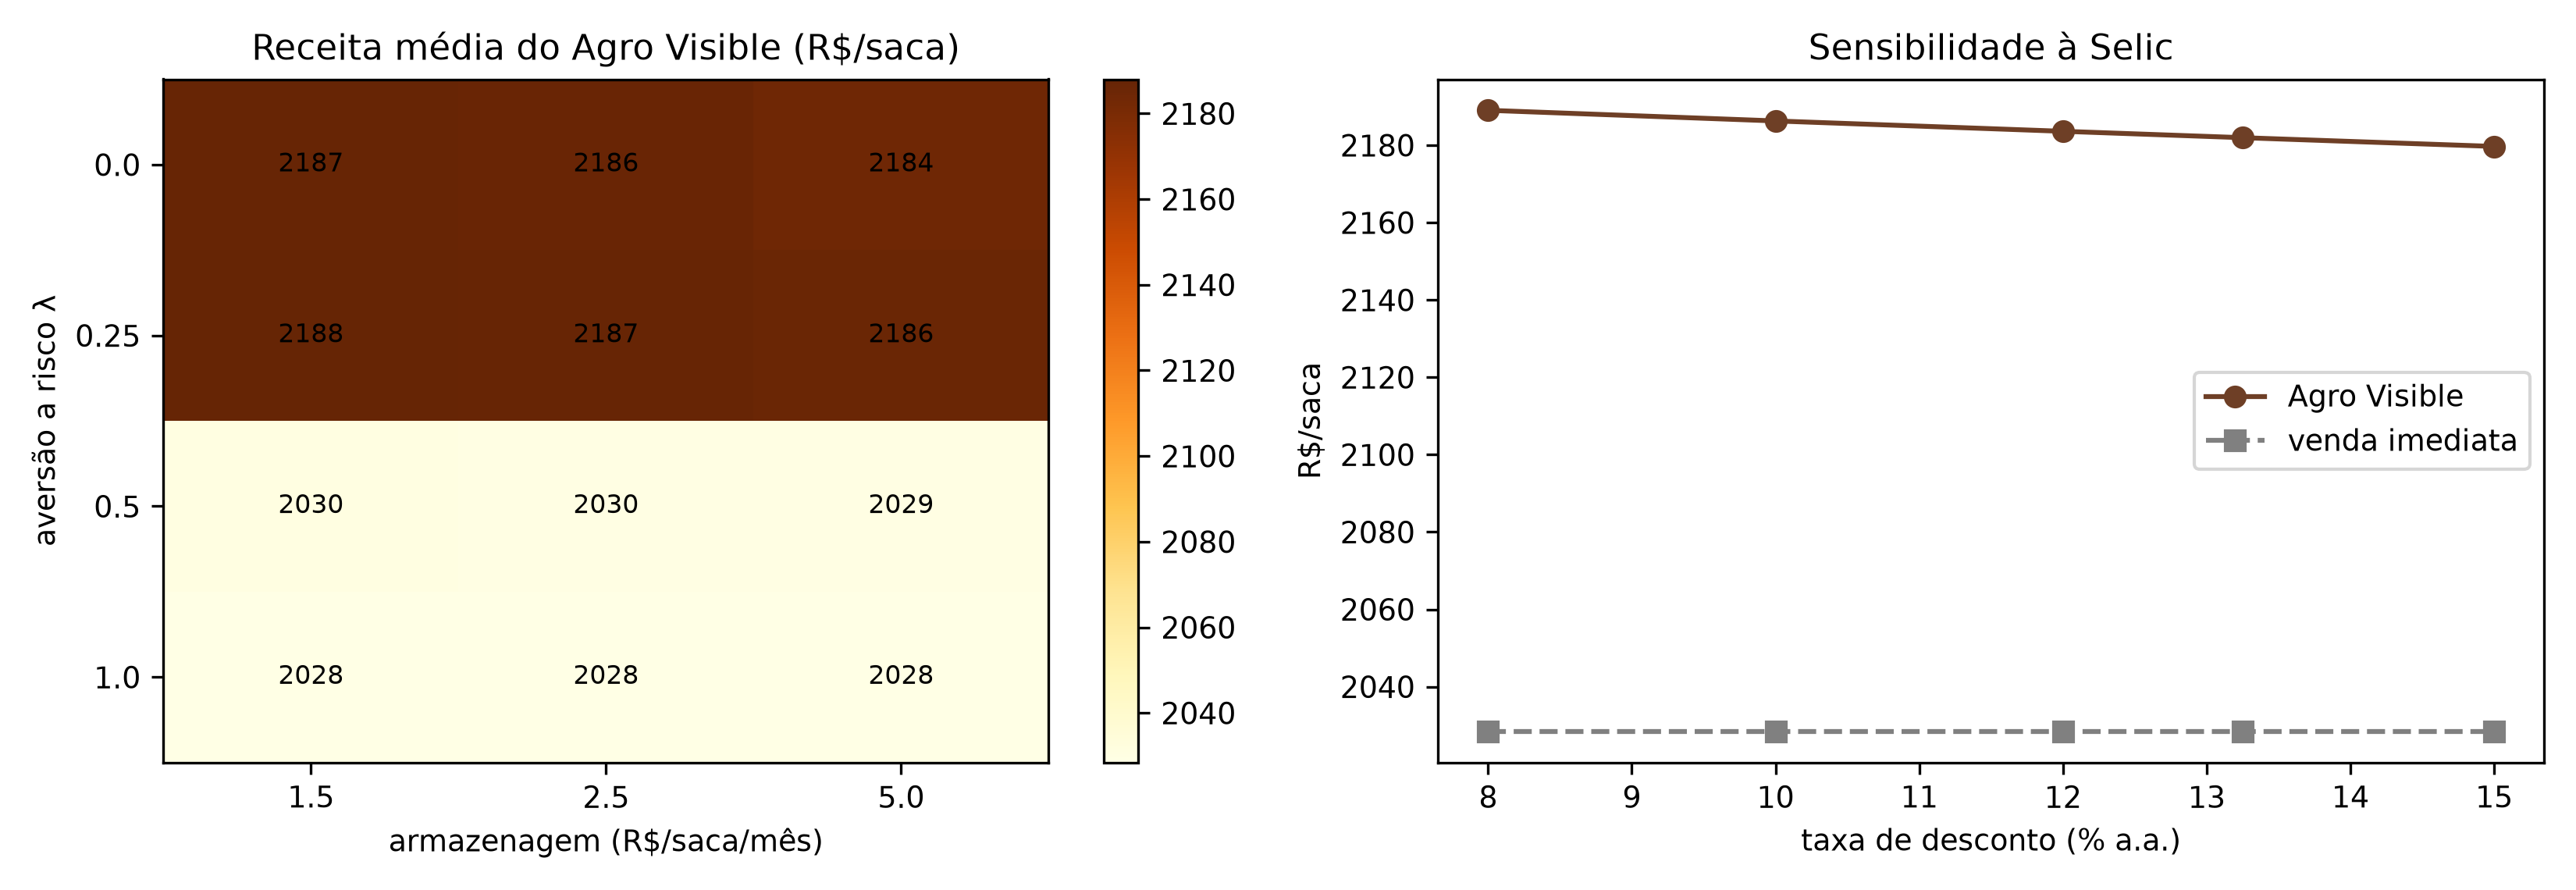
\includegraphics[width=\textwidth]{imgs/09_sensibilidade_lambda_armazenagem_selic.png}
	\fonte{Do autor (2026).}
\end{figure}

\paragraph{Taxa de desconto.} Entre 8 \% e 15 \% a.a., faixa que cobre toda a variação da Selic no período, a receita do AgroVisible move-se menos de 5 R\$/sc e nenhuma das 20 ações muda. O efeito da taxa é maior sobre a venda parcelada, que perde 31 R\$/sc na mesma faixa porque sempre carrega parte da produção por seis meses. A política é insensível à Selic porque as decisões de armazenar são tomadas quando a deriva prevista é de 10 a 20 \% em poucos meses, ordem de grandeza acima do custo de oportunidade mensal de cerca de 1 \%.

\paragraph{Armazenagem.} Entre 1,50 e 5,00 R\$/sc/mês a receita varia 2 R\$/sc e nenhuma ação muda. Com o preço da saca acima de 1\,300 R\$, a armazenagem mensal representa de 0,1 a 0,4 \% do valor, inferior ao custo de oportunidade e muito inferior à deriva prevista. Esse resultado também torna irrelevante a incerteza sobre o valor exato da tarifa de armazém, discutida no \autoref{sec:ameacas}.

\paragraph{Base e risco de base.} Com neutralidade a risco, deslocar a base esperada em 5 pontos percentuais para qualquer lado, ou dobrar o risco de base, não altera nenhuma decisão nem a receita. A razão é que a ação de \textit{hedge}, única afetada por esses parâmetros, nunca é competitiva no \textit{backtest}: com a curva de futuros aproximada pelo primeiro vencimento e o mercado em \textit{backwardation}, travar o preço futuro sempre rendia menos que vender ou armazenar descoberto. A base só passa a influenciar a política na recomendação corrente, em que a curva real por vencimento está disponível: na data de 31 de agosto de 2026, com a base em $-$26 \% contra $-$21 \% sazonal, o \textit{hedge} de um mês trava cerca de 1\,816 R\$/sc contra 1\,748 do físico e torna-se a ação recomendada para $\lambda$ entre 0,25 e 0,5.

\paragraph{Aversão a risco.} O único parâmetro que muda a política é $\lambda$. Até 0,5 a receita média permanece em 2\,079 a 2\,081 R\$/sc, mas a frequência de armazenar cai de 25 \% para 10 \% das datas: o produtor avesso a risco deixa de armazenar nas datas em que a deriva prevista é pequena diante da dispersão, e essas eram as datas de ganho marginal. Em $\lambda = 1$ o motor vende em 19 das 20 datas e a receita colapsa para a da venda imediata. A aversão a risco, portanto, não destrói o ganho da política até valores moderados; ela o concentra em menos decisões, cada uma com maior convicção. O desvio-padrão da receita entre datas, porém, cresce de 392 para 406 R\$/sc de $\lambda = 0$ a $\lambda = 1$, porque a venda imediata em um mercado volátil é, ela própria, a estratégia de maior dispersão entre datas.

\section{Custo computacional}\label{sec2:res-custo}

Em CPU, sem aceleração por GPU, o treino do modelo final levou 125 segundos; a resolução do motor de decisão para uma data, com sete camadas e 121 nós de preço, leva 2 milissegundos; o \textit{backtest} completo de 20 datas com política rolante, cerca de 120 resoluções do motor, leva 0,4 segundo. A grade de sensibilidade de 12 \textit{backtests} leva um minuto, e os 23 retreinos da ablação e do estudo de sementes levaram 35 minutos. O custo computacional da ferramenta é, portanto, compatível com execução em um computador pessoal ou em um servidor modesto de cooperativa, e a etapa cara, o treino da rede, precisa ser repetida apenas quando novos dados justificam.

\chapter{\MakeUppercase{Discussão}}\label{sec:discussao}

Este capítulo interpreta os resultados do \autoref{sec:resultados} em conjunto, extrai implicações para a pesquisa em inteligência artificial aplicada a mercados agrícolas, para os produtores e para quem constrói ferramentas de apoio à decisão, e discute as escolhas de projeto que os resultados sugerem revisar.

\section{As Questões de Pesquisa em Conjunto}\label{sec2:disc-rqs}

Lidos isoladamente, os resultados da RQ1 seriam modestos para um trabalho de previsão: a rede perde para o passeio aleatório no horizonte de um mês, perde para a curva de futuros em três meses na validação, e sua vantagem só é inequívoca no horizonte de seis meses. Lidos em conjunto com a RQ2, eles contam outra história. Uma previsão que acerta a direção em quatro de cada cinco casos no horizonte de seis meses, ainda que erre a magnitude, é suficiente para que um motor de decisão sequencial gere ganho financeiro sobre as heurísticas do produtor: 7,8\,\% sobre a venda imediata no teste cego e 6,1\,\% em quatro safras, com significância estatística nas duas amostras. A pergunta que o trabalho responde não é se a rede prevê bem, mas se a informação que ela extrai, por fraca que seja, tem valor econômico quando acoplada a uma regra de decisão que respeita custos e incerteza. A resposta, nas quatro safras analisadas, é afirmativa, com as ressalvas de amostra discutidas adiante.

Três mecanismos explicam como a estrutura de decisão sequencial mitiga os erros da previsão.

O primeiro é a \textbf{assimetria entre acerto e erro}. Quando o motor prevê recuperação a partir de um fundo e acerta, o ganho é de 10 a 30 \% em poucos meses, como em julho e agosto de 2025 e no segundo semestre de 2023. Quando prevê alta e erra, a política rolante reavalia a cada mês e vende assim que a previsão do mês seguinte deixa de justificar o carregamento, o que limita a perda na maioria dos casos. A exceção é setembro de 2022, com perda de 26 \%, quando a rede manteve a previsão de alta por dois meses consecutivos durante uma queda persistente; nesse caso a política rolante não protege, e a perda é da mesma ordem do ganho nos acertos. A assimetria média é, portanto, favorável, mas não garantida. O caso da safra 2024/25 mostra o mecanismo pelo lado positivo: em nenhuma das datas de julho a outubro de 2024 a previsão de seis meses apontava a magnitude da alta, mas a previsão de um mês foi positiva em cada uma delas, e a reavaliação mensal manteve o estoque até que ela deixasse de ser, capturando 34 a 40 \% em cada data. O motor não previu a alta; ele a seguiu mês a mês.

O segundo é a \textbf{incerteza explícita}. O motor não recebe apenas o ponto central da previsão, mas também a dispersão histórica dos resíduos por horizonte. Quando a deriva prevista é pequena diante dessa dispersão, o valor esperado de armazenar mal supera o custo de carregamento, e qualquer aversão a risco leva à venda. É por isso que, com $\lambda = 0{,}25$, a frequência de armazenar cai de 40 para 30 \% das datas sem que a receita média caia: as decisões descartadas eram as de menor convicção e menor ganho. O mesmo mecanismo, porém, torna a política frágil a partir de $\lambda = 0{,}5$: como a dispersão residual do modelo final é pequena, a penalização de risco passa a superar a deriva esperada em quase todas as datas e o motor converge para a venda imediata. O sistema converte a qualidade da previsão em largura do cone de preços, e o cone em prudência, mas o parâmetro de aversão a risco precisa ser calibrado com o produtor em uma faixa estreita, abaixo de 0,5 nesta configuração.

O terceiro é a \textbf{estrutura de gatilhos}. A saída do motor não é uma data de venda, mas uma regra: em cada mês futuro, um preço acima do qual vender é ótimo. Isso torna a política robusta a erros de magnitude da previsão, porque a venda é acionada pela realização do preço e não pela previsão dele. Um produtor que segue a regra vende quando o mercado confirma a expectativa, e não quando a rede a formula.

A RQ3 fecha o argumento. A política é insensível aos três parâmetros econômicos que a literatura de comercialização agrícola recomenda ao produtor acompanhar de perto: Selic, tarifa de armazenagem e base. Isso não significa que esses custos não importem, mas que, no regime de preços do período, a deriva prevista quando o motor decide armazenar é uma ordem de grandeza maior que o custo mensal de carregamento. Em um regime de preços baixos e juros altos a conclusão pode mudar, e o desenho do motor permite testá-lo sem alteração de código. O único parâmetro que altera a política é a aversão a risco, que é justamente o parâmetro que pertence ao produtor e não ao mercado.

Há, por fim, uma razão estrutural para que armazenar na colheita tenda a pagar, e ela ajuda a explicar por que a política ganha mesmo com previsões modestas. O preço do arábica tem sazonalidade: na mediana dos anos civis completos de 2015 a 2025, junho e julho ficam 3\,\% abaixo da média do ano, agosto 1\,\% abaixo, e novembro e dezembro 3 e 4\,\% acima, com os demais meses próximos da média. O vale coincide com a colheita, quando a oferta é abundante, e o pico com o fim do ano, quando ela se esgota. A média mensal amplifica esse padrão, com dezembro 11\,\% acima, porque a alta de 2024 dobrou o preço dentro de um mesmo ano civil, o que mostra também o quanto um único ano pode distorcer a leitura. Uma saca armazenada da colheita até o verão captura, em um ano típico, esse diferencial de 6 a 7 pontos percentuais, que supera com folga o custo de carregamento de cerca de 1\,\% ao mês. A rede aprende esse padrão, e a bienalidade e a codificação do mês são as duas variáveis de maior importância por permutação; o motor, por sua vez, só o explora quando a previsão de curto prazo não contradiz a sazonal, o que é exatamente o que se espera de uma política que combina conhecimento estrutural com informação corrente.

\section{Onde a Ferramenta Falha e Por Quê}\label{sec2:disc-falhas}

A honestidade exige tratar os resultados negativos com o mesmo cuidado dos positivos, e o trabalho tem três.

O primeiro é a simulação por safra. Quando o produtor é modelado como alguém que colhe uma vez por ano e decide a partir dali, a venda parcelada supera o AgroVisible nas duas safras cegas, 1\,837 contra 1\,807 R\$/sc, e a razão está em uma única decisão: em 1º de julho de 2024, com previsão de 21 dias negativa, o motor vendeu a saca inteira a 1\,362 R\$/sc, dois meses antes de uma alta de 84 \%. No \textit{backtest} mensal, a mesma data é apenas uma de vinte, e as dezenove seguintes compensam o erro; na simulação, a saca vendida não volta. O mecanismo que faz a política funcionar, a reavaliação mensal de um estoque existente, só opera enquanto há estoque, e uma venda total na colheita o desliga. A implicação de projeto é direta: a venda total não deveria ser a única alternativa à armazenagem total. Uma política que vende uma fração e reavalia o restante, isto é, que incorpora a venda parcelada ao motor em vez de tratá-la só como referência, preservaria a opção de participar de altas não previstas. Ela não foi implementada neste trabalho.

O segundo é a compressão das previsões. Treinada com erro quadrático em uma série próxima de um passeio aleatório, a rede aprende que a previsão de menor risco é próxima de zero, e só se afasta dela quando o sinal é forte. Em um movimento sem precedente na amostra de treino, como a alta de 2024, o sinal de seis meses não existia: as previsões de 126 dias com origem em julho a outubro de 2024 eram próximas de zero ou negativas, contra retornos realizados acima de 50 \%. O motor capturou a alta pela previsão de um mês e pela reavaliação, não porque a rede a tenha antecipado. Isso sugere prever o excedente sobre a curva de futuros em vez do retorno absoluto, o que faria a rede aprender apenas o que o mercado ainda não precifica e removeria da tarefa dela a parte que a curva já resolve.

O terceiro é a queda persistente. Em setembro e outubro de 2022, e de novo em junho de 2023, a rede previu alta no meio de uma queda que durou meses, e a política rolante, que protege contra erros isolados, não protege contra um erro repetido. A perda de setembro de 2022, de 26 \%, é da mesma ordem dos maiores ganhos. Uma revisão possível é ponderar os horizontes na interpolação pela acurácia direcional de cada um, dando ao horizonte de 126 dias, o mais confiável, maior peso na deriva dos primeiros meses; outra é condicionar a decisão de armazenar à concordância entre a previsão de curto prazo e a de seis meses. Nenhuma das duas foi implementada neste trabalho, e todas as revisões deste item são candidatas naturais a trabalhos futuros.

\section{Implicações para a Pesquisa}\label{sec2:disc-pesquisa}

O resultado central do trabalho é uma evidência empírica de que métricas estatísticas de erro são insuficientes para avaliar sistemas de inteligência artificial voltados a decisões em mercados agrícolas. Três observações sustentam essa afirmação.

Primeiro, o \textit{ranking} dos modelos por RMSE e o \textit{ranking} por valor econômico não coincidem. O ARIMA e o passeio aleatório têm o menor RMSE em 21 dias na validação, mas não carregam informação alguma para a decisão. A LSTM tem RMSE pior nesse horizonte e ainda assim gera ganho, porque acerta a direção em 63 e 126 dias. Um estudo que se encerrasse na tabela de métricas de um mês concluiria pelo modelo errado.

Segundo, a métrica que melhor antecipa o valor econômico não é o erro médio, mas a acurácia direcional no horizonte relevante para a decisão. A ablação mostra isso com clareza: os grupos de variáveis cuja remoção mais eleva o erro de 126 dias, calendário, mercado e retornos, são também os que derrubam a direção nesse horizonte, de 81 para 62 a 72 \%, enquanto a remoção de qualquer grupo é indiferente em 21 dias. A análise exploratória conta a mesma história antes do treino: a correlação das variáveis de oferta, base e calendário com o alvo cresce com o horizonte, e as de curto prazo são ruído em todos eles.

Terceiro, a avaliação econômica exige um protocolo próprio, com contabilidade de custos, referências que o agente decisor já possui e horizonte de teste que cubra mais de um regime de mercado. Os quatro trabalhos do núcleo sobre café mapeados no \autoref{sec:fundamentacao} não atendem a nenhum desses três requisitos, e a lacuna que este trabalho aponta é metodológica antes de ser algorítmica. A proposta é que estudos de previsão de preços agrícolas reportem, ao lado do RMSE, o resultado de pelo menos uma regra de decisão simples aplicada às previsões, contra pelo menos uma heurística de mercado e contra a curva de futuros quando ela existir.

Há também uma implicação sobre baselines. A curva de futuros ajustada pela base sazonal é uma referência exigente que nenhum dos trabalhos mapeados utiliza, e que na validação supera a rede neural no horizonte de três meses. Para commodities com mercado a termo líquido, essa deve ser a referência mínima de qualquer modelo preditivo, porque é a expectativa que o produtor já tem de graça.

\section{Implicações para os Produtores}\label{sec2:disc-produtores}

Para o cafeicultor, o AgroVisible oferece quatro coisas que as heurísticas usuais não oferecem.

A primeira é \textbf{disciplina}. A venda parcelada é uma boa heurística em altas e uma má heurística em quedas, e o produtor não sabe de antemão em qual regime está. A política do motor armazena quando há razão para esperar recuperação ou continuidade de alta e vende quando não há, e no \textit{backtest} de quatro safras foi a melhor estratégia não oracular em três delas e no total, perdendo apenas na safra de queda contínua, em que vender de imediato era a única política correta. A ressalva está na simulação por safra: se o produtor vende tudo na colheita por recomendação do motor, a disciplina vira rigidez, e por isso a recomendação de venda total em julho é a que mais merece ser confrontada com a leitura do próprio produtor.

A segunda é \textbf{proteção contra estocagem com margem negativa}. Ao descontar armazenagem, quebra e custo de oportunidade em cada aresta do grafo, o motor só recomenda carregar o estoque quando a deriva esperada supera o custo total de carregamento. O produtor que armazena por hábito ou por expectativa vaga não faz essa conta.

A terceira é \textbf{leitura da margem sobre o custo de produção}. Com o COE da CONAB por safra, a ferramenta informa em cada decisão a margem sobre o custo operacional efetivo e classifica o resultado esperado nas faixas de lucro supernormal a falência da gestão de custos agrícola \cite{AgroSafety2026}. No período do teste, a margem mínima foi de 74 \% e a restrição de piso não atuou; em 2023, com preços entre 800 e 1\,200 R\$/sc, ela teria atuado em mais de um terço das datas. É nos períodos de preço baixo que essa leitura importa, e é exatamente nesses períodos que o produtor tende a vender por necessidade de caixa.

A quarta é \textbf{redução da assimetria de informação}. O produtor negocia com cooperativas e tradings que acompanham a curva de futuros, a posição dos fundos e o câmbio diariamente. O AgroVisible coloca essas mesmas informações, sintetizadas em uma regra de gatilho por mês, à disposição de quem vende uma saca.

Duas advertências acompanham essas implicações. A ferramenta não substitui a leitura do produtor sobre sua própria situação de caixa, e a restrição de piso sobre o COE foi mantida desligada justamente porque forçar o carregamento quando o preço está abaixo do custo pode ser pior que vender. E a política é calibrada para o mercado físico de referência, não para o preço de balcão de uma cooperativa específica, cuja base local pode diferir da modelada.

\section{Implicações para Construtores de Ferramentas}\label{sec2:disc-tools}

A experiência de construir o AgroVisible sugere sete diretrizes de engenharia para plataformas de apoio à decisão voltadas a cooperativas e empresas agrícolas.

\begin{alineas}
	\item \textbf{Desacoplar previsão e decisão.} A interface entre os dois módulos é um vetor de médias e um de desvios por horizonte. Isso permitiu trocar o alvo da rede, retreiná-la com sementes diferentes e rodar ablações sem tocar no motor, e permitirá substituir a LSTM por qualquer estimador futuro. Ferramentas que embutem a previsão na regra de decisão perdem essa flexibilidade.
	\item \textbf{Exigir incerteza do módulo preditivo.} Um ponto central sem dispersão obriga o motor a tratar todas as previsões como igualmente confiáveis. A dispersão residual por horizonte é barata de calcular e é o que torna a aversão a risco operacional.
	\item \textbf{Entregar regras, não datas.} O gatilho de venda por mês é mais útil e mais robusto que uma recomendação pontual, porque o produtor o executa contra o preço observado. A interface da ferramenta deve exibir a regra, o cone de preços e a distribuição do mês de venda, e não apenas a ação de hoje.
	\item \textbf{Tratar a data de disponibilidade como parte do dado.} O relatório de posições de fundos refere-se a uma terça-feira e sai na sexta; os preços de insumos do mês saem dias depois do fechamento. Ancorar cada série na data em que ela ficou conhecida, e não na data a que se refere, evitou vazamentos que só foram detectados por auditoria explícita do pipeline.
	\item \textbf{Comparar com o que o usuário já tem.} A curva de futuros é a expectativa gratuita do produtor com acesso à bolsa. Uma ferramenta que não a supera não agrega valor preditivo, ainda que supere baselines estatísticos, e deve dizer isso ao usuário em vez de esconder atrás de um RMSE.
	\item \textbf{Validar por \textit{backtest} rolante em mais de um regime.} Vinte decisões em duas safras de alta não distinguem uma política boa de uma sortuda. Dobrar a amostra com um período de queda mudou a leitura de várias estratégias, inclusive da venda parcelada, e é o mínimo para qualquer afirmação de ganho.
	\item \textbf{Dimensionar para o computador do usuário.} O motor resolve uma decisão em milissegundos e o treino da rede leva pouco mais de um minuto em CPU. Cooperativas não precisam de infraestrutura de nuvem para operar a ferramenta, e o retreino, que neste estudo foi feito uma única vez, pode ser executado a cada safra ou a cada mês em um servidor comum, com a ressalva de que cada retreino exige repetir a verificação com várias sementes.
	\item \textbf{Começar pela rede menor.} A configuração inicial, de 64 unidades, parecia modesta e estava sobreajustada a 3\,940 janelas de treino; a busca mostrou que metade das unidades e o dobro do \textit{dropout} melhoram o erro de seis meses em 19\,\% na média de cinco sementes. Em séries agrícolas, com poucas safras de histórico, a capacidade da rede deve ser dimensionada pela amostra, não pela convenção da literatura, e a busca de hiperparâmetros deve ser verificada com várias sementes, porque uma semente favorável pode exagerar o ganho.
\end{alineas}

Uma última observação diz respeito à origem dos parâmetros econômicos. A tarifa de armazenagem e a quebra técnica foram estimativas do desenvolvimento, sem documento de referência, e a análise de sensibilidade mostrou que a decisão é insensível a elas na faixa plausível. Esse é um resultado útil para quem constrói ferramentas semelhantes: nem todo parâmetro precisa ser levantado com precisão antes de a ferramenta ser útil, e a análise de sensibilidade é a forma de descobrir quais precisam.

\chapter{\MakeUppercase{Ameaças à Validade}}\label{sec:ameacas}

Este capítulo discute as ameaças à validade do estudo segundo a taxonomia de \citeonline{Wohlin2012}, que distingue validade de conclusão, de construção, interna e externa. Para cada ameaça são descritos a origem, a mitigação adotada e o que permanece como limitação. Várias das ameaças foram identificadas durante o desenvolvimento e motivaram correções no pipeline; essas correções são registradas aqui porque documentam o que o protocolo final evita e o que ele ainda não evita.

\section{Validade de Conclusão}\label{sec2:amc-conclusao}

A validade de conclusão diz respeito à capacidade de inferir, com a estatística adequada, que existe relação entre o tratamento e o resultado.

\paragraph{Tamanho e tipicidade da amostra de decisões.} A ameaça mais séria do estudo é o número de decisões avaliadas. O teste cego tem 20 datas em duas safras, ambas de preço recorde; o consolidado com a validação tem 38 datas em quatro safras. Com essa amostra, a diferença entre o AgroVisible e a venda imediata não é significativa ao nível de 5\,\% no teste isolado e fica na margem ($p = 0{,}066$) no consolidado. Apenas a diferença contra a venda parcelada atinge significância ($p = 0{,}018$) com 38 datas. A mitigação foi ampliar a amostra ao período de validação, reportar intervalos de confiança por \textit{bootstrap} ao lado dos p-valores, e apresentar a fração do ganho do oráculo capturada, que é menos sensível ao nível de preços que a diferença em reais. A limitação permanece: as conclusões sobre ganho financeiro devem ser lidas como evidência favorável, não como demonstração.

\paragraph{Estrutura da diferença pareada.} O teste de Wilcoxon penaliza a política do motor por um motivo estrutural: na maioria das datas ele vende imediatamente e a diferença é exatamente zero, de modo que o ganho médio vem de poucas decisões com retorno alto. A fração de datas com diferença positiva contra a venda imediata é de 34\,\%, o que um leitor apressado tomaria por evidência de política ruim. A mitigação foi reportar, além do p-valor, a média, o intervalo de confiança e a decomposição por data, e explicar no texto a origem da mediana nula.

\paragraph{Variabilidade de treino da rede.} Diferenças de RMSE entre modelos podem ser ruído de inicialização. A mitigação foi treinar o modelo completo com cinco sementes e cada configuração da ablação com três, e interpretar apenas as diferenças maiores que o desvio entre sementes. Com esse critério, a vantagem da curva de futuros em 63 dias é robusta e a de 21 dias não é, e apenas dois grupos da ablação têm efeito interpretável no horizonte de 126 dias. A limitação é que três sementes por configuração ainda são poucas para efeitos pequenos, e a ablação deve ser lida como indicativa.

\paragraph{Múltiplas comparações.} O estudo compara sete estratégias, seis configurações de ablação e uma grade de sensibilidade, e não aplica correção para múltiplas comparações. As afirmações de significância referem-se a duas comparações pré-especificadas na RQ2, contra a venda imediata e contra a parcelada; as demais são descritivas.

\section{Validade de Construção}\label{sec2:amc-construcao}

A validade de construção diz respeito à aderência entre os conceitos que se pretende medir e as medidas efetivamente usadas.

\paragraph{Preço do produtor.} O sistema usa o indicador CEPEA/ESALQ como o preço que o produtor de Minas Gerais recebe. O indicador é a média de negócios nas praças de Minas e São Paulo, e o preço de balcão de uma cooperativa específica difere dele por um diferencial local que não é modelado. A consequência é que a base regional no sentido estrito, entre indicador e cooperativa, não é capturada; o que o sistema modela é a base entre o físico de referência e o futuro. Para um produtor cujo diferencial local é estável, a política é a mesma; para um cujo diferencial varia, há um risco de base adicional não contabilizado. Não há série pública que permita mitigar essa ameaça.

\paragraph{Instrumento de \textit{hedge}.} O contrato ICF da B3, referência doméstica, não tem série histórica pública com profundidade suficiente, e o contrato \textit{Coffee C} da ICE convertido pela PTAX foi usado como \textit{proxy}. O \textit{hedge} modelado não inclui margem de garantia nem ajuste diário, e assume caixa disponível para chamadas de margem sem descontar seu custo financeiro. O custo operacional de 10 R\$/sc foi tomado de material didático \cite{AgroSafety2026} sem decomposição em taxa de operação, emolumentos e registro. Como o motor nunca escolheu o \textit{hedge} no \textit{backtest}, essas simplificações não afetam os resultados de receita reportados, mas afetariam uma avaliação em que o \textit{hedge} fosse competitivo. No \textit{backtest}, a curva de futuros foi aproximada pelo primeiro vencimento porque a fonte de dados descarta contratos vencidos; a curva real por vencimento só passou a ser acumulada em setembro de 2026, e é ela que, na recomendação corrente, torna o \textit{hedge} de um mês a ação recomendada para aversão a risco moderada.

\paragraph{Custos de carregamento.} A tarifa de armazenagem de 2,50 R\$/sc/mês e a quebra técnica de 0,2\,\%/mês foram estimativas do desenvolvimento, sem documento de cooperativa ou armazém geral que as sustente. A mitigação foi a análise de sensibilidade, que mostrou receita e política insensíveis à armazenagem entre 1,50 e 5,00 R\$/sc/mês. A quebra técnica não foi variada. O custo de oportunidade usa a meta Selic como taxa livre de risco, sem considerar que o produtor pode ter custo de capital superior, por dívida de custeio, ou inferior, por aplicação a taxas de poupança; a sensibilidade entre 8 e 15\,\% a.a. cobre a faixa plausível e não altera decisões.

\paragraph{Custo de produção.} O COE por safra vem da planilha da CONAB para Guaxupé, sistema semiadensado de alta tecnologia e agricultura familiar, e não do custo real de um produtor específico. Duas safras dessa praça não têm COT e custo total na planilha. O COE entra no motor como piso opcional e como informação de margem, e a restrição de piso não atuou em nenhuma data do teste; portanto, a imprecisão do COE não afeta a receita reportada, apenas a classificação de margem exibida ao produtor.

\paragraph{Métricas preditivas.} RMSE e MAE são calculados sobre log-retornos e o MAPE sobre o preço reconstruído, o que os torna comparáveis entre horizontes mas não diretamente comparáveis com trabalhos que reportam erro sobre o preço em nível. A acurácia direcional foi acrescentada porque é a métrica que melhor antecipa o valor econômico, mas ela ignora a magnitude e trata um acerto de 1\,\% como igual a um de 30\,\%.

\paragraph{Heurísticas de comparação.} A venda parcelada foi implementada como seis parcelas mensais iguais, a média móvel como cruzamento da média de 63 dias e a meta de margem como 130\,\% do COE. Produtores reais usam variantes dessas regras com parâmetros distintos, e uma variante mais bem calibrada poderia reduzir a vantagem do motor. As heurísticas não foram otimizadas sobre os dados de teste, o que seria injusto com elas em sentido oposto.

\section{Validade Interna}\label{sec2:amc-interna}

A validade interna diz respeito à ausência de fatores não controlados que possam explicar o resultado no lugar do tratamento. Em um estudo de séries temporais, o fator dominante é o vazamento de informação futura.

\paragraph{Partição temporal.} A partição é estritamente cronológica por ano-safra, e o padronizador das variáveis é ajustado apenas no treino. Duas correções foram necessárias durante o desenvolvimento. Na primeira versão, as janelas de entrada eram construídas apenas dentro de cada conjunto, o que descartava os 62 primeiros dias da validação e do teste e fazia a primeira previsão partir de um preço quatro meses posterior ao último conhecido; a correção permitiu que a janela de entrada cruzasse a fronteira do conjunto anterior, por ser histórico já conhecido. Na primeira tentativa dessa correção o alvo também cruzou a fronteira, o que rotularia os últimos 126 dias do treino com preços da validação; isso foi detectado e corrigido antes do retreino, descartando como origem de amostra as últimas 126 datas de cada conjunto.

\paragraph{Data de disponibilidade das fontes.} O relatório de posições de fundos e os preços mensais de insumos foram inicialmente alinhados pela data de referência, o que usava informação ainda não publicada. Ambos foram reancorados na data de divulgação. Os acumulados de chuva foram calculados no calendário civil antes do recorte para dias úteis. As demais séries são diárias e alinhadas pelo último valor conhecido. Não há garantia de que nenhum vazamento sutil permaneça, mas os canais conhecidos foram auditados.

\paragraph{Estatísticas de base.} A base sazonal esperada e o risco de base foram, em uma primeira versão, estimados até o fim dos dados disponíveis, o que incluía a validação e o teste. A correção restringiu a estimativa ao período de treino. Essa correção foi feita antes dos experimentos reportados.

\paragraph{Viés no período de validação.} O \textit{backtest} estendido às safras 2022/23 e 2023/24 usa a dispersão residual e a parada antecipada calibradas nesses mesmos dados. O viés é favorável à rede e de magnitude pequena, porque a dispersão residual afeta apenas a largura do cone e não a direção da previsão, mas existe. Os resultados dessas duas safras são reportados separadamente dos do teste cego e o viés é declarado na tabela.

\paragraph{Modelo salvo desatualizado.} Durante o desenvolvimento, o caderno de previsão carregava o modelo do disco quando ele existia e chegou a produzir métricas com um modelo anterior à mudança nas janelas. Os experimentos reportados foram executados após retreino do zero, com semente fixa, e as métricas reproduziram exatamente as do dossiê de referência.

\paragraph{Seleção do modelo final.} A configuração da rede (unidades, dropout, janela, taxa de aprendizado) foi fixada a priori, sem busca em validação, o que evita sobreajuste ao conjunto de validação por seleção de hiperparâmetros. A semente 42 do modelo final ficou dentro de um desvio-padrão da média das cinco sementes em todas as métricas, o que afasta a hipótese de que o resultado seja um sorteio favorável.

\paragraph{Sobreajuste.} O RMSE de treino é de cerca de 0,03 contra 0,11 a 0,19 na validação, e a ablação mostra que remover três grupos de variáveis melhora o erro de longo prazo. O modelo completo está sobreajustado. Isso não invalida os resultados, que são medidos fora da amostra, mas indica que o ganho reportado é provavelmente um piso do que a arquitetura pode entregar.

\section{Validade Externa}\label{sec2:amc-externa}

A validade externa diz respeito à generalização dos resultados para além das condições do estudo.

\paragraph{Regime de mercado.} As quatro safras avaliadas cobrem uma queda de 40\,\%, uma recuperação a partir de um fundo, uma alta de 84\,\% e um platô alto. Faltam períodos de preço lateral prolongado e de preço baixo persistente, como 2018 a 2019, em que a política pode se comportar de forma diferente e em que a restrição de piso sobre o COE passaria a atuar. A geada de 2021 está no treino, não na avaliação. Uma avaliação em janela rolante ao longo de toda a série, retreinando a rede a cada safra, é o desenho que responderia a essa ameaça, e não foi executada por custo computacional e de tempo.

\paragraph{Outras praças cafeeiras.} O modelo foi treinado sobre o indicador do arábica em Minas e São Paulo, com clima de três regiões mineiras e paulistas. A transferência para o Espírito Santo, onde predomina o robusta, exigiria trocar o alvo pelo indicador do robusta, o instrumento de \textit{hedge} pelo contrato de conilon da B3 e as regiões climáticas, e reestimar a base. A arquitetura permite isso sem alteração de código, mas nenhum resultado deste trabalho se transfere diretamente.

\paragraph{Outras culturas.} A estrutura do motor de decisão é agnóstica à cultura: qualquer commodity armazenável com mercado a termo se ajusta ao mesmo processo de decisão. A transferência para grãos como milho e soja, que têm sazonalidade, custos de armazenagem e liquidez diferentes, exigiria novas fontes, novas variáveis e nova calibração, e a decisão de manter o escopo em uma única cultura foi tomada justamente porque cada cultura adicional multiplica esse trabalho.

\paragraph{Escala do produtor.} O \textit{backtest} avalia uma saca hipotética e assume que a venda não afeta o preço. Para um produtor pequeno essa hipótese é razoável; para uma cooperativa que comercializa milhões de sacas, o volume influencia a base local e a política precisaria de um modelo de impacto de mercado. O \textit{hedge} também é avaliado por saca, quando o contrato mínimo da B3 é de 100 sacas, o que exclui produtores muito pequenos da ação de proteção sem uma cooperativa intermediária.

\paragraph{Liquidez e execução.} O modelo assume que o produtor consegue vender a qualquer momento ao preço do indicador, sem custo de transação nem prazo de liquidação. Na prática, a venda física envolve classificação do lote, negociação com o comprador e prazo de pagamento, e o preço obtido pode diferir do indicador do dia. Essa hipótese de liquidez perfeita é comum na literatura e é retomada nas limitações do \autoref{sec:conclusao}.

\paragraph{Dependência de fontes de dados.} O indicador CEPEA exige download manual porque o portal bloqueia acesso automatizado; os contratos vencidos da ICE são descartados pela fonte gratuita; o contrato de robusta de Londres foi deslistado durante o projeto. Uma ferramenta em produção dependeria de acesso a dados pagos ou de acordo institucional, e a reprodutibilidade do estudo depende dos arquivos brutos preservados no repositório.

%\chapter{\MakeUppercase{Conclusão}}\label{sec:conclusao}

Este trabalho construiu e avaliou o AgroVisible, uma ferramenta que acopla uma rede LSTM alimentada por variáveis exógenas a um processo de decisão de Markov resolvido por programação dinâmica para prescrever quando vender o café arábica colhido. A avaliação seguiu um protocolo de estudo empírico, com questões de pesquisa definidas a priori, partição cronológica estrita, \textit{backtest} em safras cegas e análise de sensibilidade.

\section{Síntese das respostas}

\paragraph{RQ1.} A rede, na configuração final de 32 e 16 unidades com \textit{dropout} 0,4, escolhida por busca em validação e verificada com cinco sementes, não supera o passeio aleatório no horizonte de 21 dias e perde para a curva de futuros no de 63 dias na validação. No horizonte de 126 dias ela vence todas as referências nos dois conjuntos, e no teste cego vence as duas referências em 63 e 126 dias, com acerto direcional de 76 e 77\,\%. O valor preditivo está na direção de médio prazo, não na magnitude nem no curto prazo. A análise exploratória, a importância por permutação e a ablação convergem: o sinal vem da oferta, da base físico-futuro, do calendário e da bienalidade, cresce com o horizonte, e as variáveis de curto prazo são ruído. Cinco dos seis grupos contribuem no horizonte de seis meses, com calendário, mercado e retornos como essenciais, e nesta configuração os insumos não contribuíram.

\paragraph{RQ2.} No \textit{backtest} cego de vinte decisões mensais, a política obteve 2\,186 reais por saca contra 2\,028 da venda imediata e 2\,001 da venda parcelada, ganhos de 7,8 e 9,2\,\%, significativos a 5\,\%. Em quatro safras, de 2022 a 2026, o ganho foi de 6,1 e 9,0\,\%, também significativo, e a política capturou 94\,\% do valor do oráculo, sendo a melhor estratégia não oracular em três das quatro safras. A ação de \textit{hedge} nunca foi escolhida no \textit{backtest}, porque o mercado esteve em \textit{backwardation}, mas passa a ser recomendada na data mais recente, com a curva real por vencimento, para aversão a risco moderada. A simulação por safra, com uma única decisão na colheita, mostrou o limite da política: uma venda total em 1º de julho de 2024 perdeu a alta inteira daquela safra, e nas duas safras cegas a venda parcelada ficou à frente.

\paragraph{RQ3.} A política é insensível à taxa de desconto entre 8 e 15\,\% ao ano, à tarifa de armazenagem entre 1,50 e 5,00 reais por saca ao mês e a choques de base, porque a deriva prevista nas datas em que o motor armazena é uma ordem de grandeza maior que o custo de carregamento. O único parâmetro que altera a política é a aversão a risco: até $\lambda = 0{,}25$ ela preserva a receita e reduz a frequência de armazenar; a partir de $\lambda = 0{,}5$ converge para a venda imediata.

Em síntese, a hipótese do trabalho foi confirmada nas condições estudadas: uma previsão que acerta a direção em seis meses, mesmo errando a magnitude e o curto prazo, gera valor econômico quando acoplada a uma regra de decisão que respeita custos e incerteza. A contribuição principal não é uma arquitetura mais acurada, mas a demonstração de que a avaliação de um modelo preditivo para decisões de comercialização precisa ir além da métrica de erro, e de que a mesma rede pode ser considerada fraca por uma tabela de RMSE e útil por um \textit{backtest} de receita.

\section{Limitações}

As limitações mais importantes foram tratadas no \autoref{sec:ameacas} e são resumidas aqui. A amostra de avaliação é pequena, vinte decisões cegas e trinta e oito no total, em um período de preços recordes, e os intervalos de confiança do ganho são largos. A arquitetura e a dispersão residual foram selecionadas no conjunto de validação, e a semente do modelo final é favorável, de modo que as métricas de validação são otimistas. O horizonte de 21 dias não tem valor preditivo, e a política depende dele como primeira porta de decisão, o que produziu a venda prematura de julho de 2024. A variável de geada é inerte, e o choque climático mais relevante do período de treino não está representado nos dados de entrada. Os custos de armazenagem e quebra são estimativas sem documento de referência, ainda que a sensibilidade mostre que não alteram a decisão. O \textit{hedge} é modelado sem margem de garantia nem ajuste diário, com um contrato estrangeiro como \textit{proxy} do doméstico e, no \textit{backtest}, com curva plana. E o preço do produtor é aproximado pelo indicador CEPEA/ESALQ, sem a base local de cada cooperativa.

\section{Trabalhos futuros}

Os resultados apontam extensões em três direções.

Na previsão, a mais promissora é prever o excedente sobre a curva de futuros em vez do retorno absoluto, deixando à rede apenas o que o mercado ainda não precifica, e ponderar os horizontes na interpolação pela acurácia direcional de cada um. A variável de geada deve ser redefinida, com limiar de 5\,$^{\circ}$C ou como anomalia de temperatura em relação à climatologia do mês, e variáveis de oferta ainda não coletadas, como os estoques certificados da bolsa e as estimativas de safra da CONAB e do USDA, devem ser incorporadas. Uma avaliação em janela rolante ao longo de toda a série, retreinando a rede a cada safra, responderia à ameaça de regime de mercado.

Na decisão, a venda parcelada deve entrar no motor como ação, e não apenas como referência: vender uma fração e reavaliar o restante preservaria a opção de participar de altas não previstas, que foi o que a venda total na colheita de 2024 destruiu. A compra de opções de venda, que limita a perda sem travar o ganho, é a extensão natural da ação de \textit{hedge}, e exige modelar prêmio e volatilidade implícita. O \textit{hedge} em si deve incorporar margem de garantia e ajuste diário.

Na ferramenta, o passo seguinte é uma aplicação móvel ou web que entregue ao produtor, mensalmente, a ação do dia, o gatilho de venda por mês e a classificação de margem sobre o custo de produção, com os parâmetros econômicos e a aversão a risco configuráveis. A estrutura do motor é agnóstica à cultura, e a extensão a outras commodities armazenáveis com mercado a termo, como o milho e a soja, exige novas fontes, novas variáveis e nova calibração, mas não um novo método.


%==============================================================================
% Bibliografia

% Carrega o estilo para referências ABNT
\bibliographystyle{abntex2-alf}            

% Alterando informações do estilo de citação.
% Como estamos usando uma versão alterada, essas opções são necessárias.
% Et al. em itálico
\citeoption{abnt-etal-text=it}

% Até 3 autores antes do et al.
\citeoption{abnt-etal-cite=3}

% Colocar s.d. na falta de um ano de publicação
\citeoption{abnt-missing-year=sd}

% Altera o estilo de citação para (Autor, ano)
% A opção abnt-cite-style=AuthorYEAR está quebrada; essa é equivalente.
\citeoption{abnt-nbr10520=1988}
\citeoption{abnt-and-type=e}


% Comando necessário para corrigir o título das referências.
% Para o estilo ABNT, esse comando SEMPRE deve ser
% chamado antes do \bibliography
\referencias
% Adiciona as referência em bibtex 
\bibliography{refbib}

%==============================================================================
% Outros elementos pós-textuais

% Glossário
%\glossario

% Anexos e apêndices
% Os anexos devem ser includios antes
% e utilizar \input ao invés de \include, para não criar uma nova página
% Anexos
%\anexo{Lorem Ipsum}\label{anex:lorem1}

Lorem ipsum dolor sit amet, consectetur adipiscing elit. Vivamus semper, libero egestas pellentesque vulputate, velit felis commodo ante, vel bibendum velit turpis eu felis. Donec viverra quam nisi, vel tincidunt enim tristique interdum. Integer tincidunt a lectus vel porttitor. Nulla venenatis vitae enim ut semper. Nunc in sagittis massa, sit amet dapibus quam. Mauris cursus, ligula ac pretium imperdiet, lectus libero egestas mi, quis tristique leo urna nec erat. In vitae dui maximus, imperdiet massa euismod, auctor enim. Morbi urna odio, accumsan quis magna id, fringilla gravida purus. Aenean facilisis est nisi, nec porttitor purus ullamcorper ut. Proin ac risus congue, aliquet elit in, cursus est.

Vivamus lorem diam, molestie ut ultrices at, feugiat quis tortor. Mauris feugiat, augue at molestie malesuada, purus erat sagittis tellus, sit amet posuere lacus nisl non eros. Sed enim justo, sagittis id elementum quis, commodo ut nibh. Aenean mauris odio, efficitur vel purus sit amet, molestie pharetra arcu. Nunc vel eros sodales, aliquam diam eu, rutrum nisi. Morbi non scelerisque diam. Suspendisse sed dapibus mi, ut sagittis nunc. Praesent ornare, est in rutrum dapibus, tortor massa ornare dolor, at ullamcorper metus augue et ipsum. Sed ut nulla in dolor aliquet faucibus. Quisque rhoncus auctor tellus eu lobortis. Proin rhoncus nisi sit amet nibh tempor hendrerit.\footnote{Lorem ipsum dolor sit amet, consectetur adipiscing elit. Vivamus semper, libero egestas pellentesque vulputate, velit felis commodo ante, vel bibendum velit turpis eu felis. Donec viverra quam nisi, vel tincidunt enim tristique interdum. Integer tincidunt a lectus vel porttitor.}
%\anexo{Lorem Ipsum pt. 2}\label{anex:lorem2}

Aliquam tempus vehicula risus sit amet consequat. Donec eu mattis lorem. Maecenas tincidunt a massa ut ultricies. Ut id lacus sapien. Suspendisse ac auctor lectus. Maecenas vehicula sagittis metus, eget luctus ipsum imperdiet at. Nullam eu vestibulum leo. Fusce mauris ligula, consequat ut felis a, ornare bibendum quam. Maecenas posuere sem sit amet volutpat interdum. Integer aliquet bibendum luctus. Nulla non viverra eros. Fusce egestas scelerisque augue ac tempor.


Aliquam tempus vehicula risus sit amet consequat. Donec eu mattis lorem. Maecenas tincidunt a massa ut ultricies. Ut id lacus sapien. Suspendisse ac auctor lectus. Maecenas vehicula sagittis metus, eget luctus ipsum imperdiet at. Nullam eu vestibulum leo. Fusce mauris ligula, consequat ut felis a, ornare bibendum quam. Maecenas posuere sem sit amet volutpat interdum. Integer aliquet bibendum luctus. Nulla non viverra eros. Fusce egestas scelerisque augue ac tempor.


Aliquam tempus vehicula risus sit amet consequat. Donec eu mattis lorem. Maecenas tincidunt a massa ut ultricies. Ut id lacus sapien. Suspendisse ac auctor lectus. Maecenas vehicula sagittis metus, eget luctus ipsum imperdiet at. Nullam eu vestibulum leo. Fusce mauris ligula, consequat ut felis a, ornare bibendum quam. Maecenas posuere sem sit amet volutpat interdum. Integer aliquet bibendum luctus. Nulla non viverra eros. Fusce egestas scelerisque augue ac tempor.

% Apendices
%\apendice{O que são apêndices}\label{apen:apendice}

Um apêndice é um suporte elucidativo e ilustrativo do texto principal. Sua função é agrupar elementos que são úteis à compreensão do texto e que, no entanto, podem ser apresentados à parte sem prejuízo à compreensão. É útil para a apresentação de modelagens, diagramas extensos, listagens de código-fonte de programas e demais elementos que o autor julgar necessário à complementação do tema abordado no texto principal.


% Índice
%\indice


%==============================================================================
% Fim do documento
%==============================================================================
\end{document}
